%%%%%%%%%%%%%%%%%%%%%%% file template.tex %%%%%%%%%%%%%%%%%%%%%%%%%
%
% This is a general template file for the LaTeX package SVJour3
% for Springer journals.          Springer Heidelberg 2010/09/16
%
% Copy it to a new file with a new name and use it as the basis
% for your article. Delete % signs as needed.
%
% This template includes a few options for different layouts and
% content for various journals. Please consult a previous issue of
% your journal as needed.
%
%%%%%%%%%%%%%%%%%%%%%%%%%%%%%%%%%%%%%%%%%%%%%%%%%%%%%%%%%%%%%%%%%%%
%
% First comes an example EPS file -- just ignore it and
% proceed on the \documentclass line
% your LaTeX will extract the file if required
%\begin{filecontents*}{example.eps}
%%!PS-Adobe-3.0 EPSF-3.0
%%%BoundingBox: 19 19 221 221
%%%CreationDate: Mon Sep 29 1997
%%%Creator: programmed by hand (JK)
%%%EndComments
%gsave
%newpath
%  20 20 moveto
%  20 220 lineto
%  220 220 linetof
%  220 20 lineto
%closepath
%2 setlinewidth
%gsave
%  .4 setgray fill
%grestore
%stroke
%grestore
%\end{filecontents*}
%
\RequirePackage{fix-cm}
%
%\documentclass{svjour3}                     % onecolumn (standard format)
%\documentclass[smallcondensed]{svjour3}     % onecolumn (ditto)
\documentclass[smallextended]{svjour3}       % onecolumn (second format)
%\documentclass[twocolumn]{svjour3}          % twocolumn
%
\smartqed  % flush right qed marks, e.g. at end of proof
%
\usepackage{graphicx}
%
% \usepackage{mathptmx}      % use Times fonts if available on your TeX system
%
% insert here the call for the packages your document requires
%\usepackage{latexsym}
% etc.
%
% please place your own definitions here and don't use \def but
% \newcommand{}{}
%
% Insert the name of "your journal" with
% \journalname{myjournal}
%


\usepackage{bm}
\usepackage{amssymb,amsmath,times,subfigure,tabularx,booktabs,colortbl,multirow,threeparttable}
\usepackage{subfigure}
%\usepackage[notref,notcite]{showkeys}  % use this to temporarily show labels
\usepackage[colorlinks=true, pdfstartview=FitV, linkcolor=black, citecolor= black, urlcolor= black]{hyperref}
%\usepackage{overcite}
\usepackage{footnpag}			      	% make footnote symbols restart on each page

\usepackage{color}
\newcommand{\hilight}[1]{\colorbox{green}{#1}}

\newtheorem{prop}{Proposition}

\newcommand{\abs}{\mathop{\mathrm{abs}}\nolimits}
\newcommand{\diag}{\mathop{\mathrm{diag}}\nolimits}
\newcommand{\norm}[1]{\ensuremath{\left\| #1 \right\|}}
\newcommand{\bracket}[1]{\ensuremath{\left[ #1 \right]}}
\newcommand{\braces}[1]{\ensuremath{\left\{ #1 \right\}}}
\newcommand{\parenth}[1]{\ensuremath{\left( #1 \right)}}
\newcommand{\pair}[1]{\ensuremath{\langle #1 \rangle}}
\newcommand{\met}[1]{\ensuremath{\langle\langle #1 \rangle\rangle}}
\newcommand{\refeqn}[1]{(\ref{eqn:#1})}
\newcommand{\reffig}[1]{Fig. \ref{fig:#1}}
\newcommand{\tr}[1]{\mathrm{tr}\ensuremath{\negthickspace\bracket{#1}}}
\newcommand{\trs}[1]{\mathrm{tr}\ensuremath{[#1]}}
\newcommand{\ave}[1]{\mathrm{E}\ensuremath{[#1]}}
\newcommand{\deriv}[2]{\ensuremath{\frac{\partial #1}{\partial #2}}}
\newcommand{\SO}{\ensuremath{\mathsf{SO(3)}}}
\newcommand{\T}{\ensuremath{\mathsf{T}}}
\renewcommand{\L}{\ensuremath{\mathsf{L}}}
\newcommand{\so}{\ensuremath{\mathfrak{so}(3)}}
\newcommand{\SE}{\ensuremath{\mathsf{SE(3)}}}
\newcommand{\se}{\ensuremath{\mathfrak{se}(3)}}
\renewcommand{\Re}{\ensuremath{\mathbb{R}}}
\newcommand{\aSE}[2]{\ensuremath{\begin{bmatrix}#1&#2\\0&1\end{bmatrix}}}
\newcommand{\ase}[2]{\ensuremath{\begin{bmatrix}#1&#2\\0&0\end{bmatrix}}}
\newcommand{\D}{\ensuremath{\mathbf{D}}}
\renewcommand{\d}{\ensuremath{\mathfrak{d}}}
\newcommand{\Sph}{\ensuremath{\mathsf{S}}}
\renewcommand{\S}{\Sph}
\newcommand{\J}{\ensuremath{\mathbf{J}}}
\newcommand{\Ad}{\ensuremath{\mathrm{Ad}}}
\newcommand{\intp}{\ensuremath{\mathbf{i}}}
\newcommand{\extd}{\ensuremath{\mathbf{d}}}
\newcommand{\hor}{\ensuremath{\mathrm{hor}}}
\newcommand{\ver}{\ensuremath{\mathrm{ver}}}
\newcommand{\dyn}{\ensuremath{\mathrm{dyn}}}
\newcommand{\geo}{\ensuremath{\mathrm{geo}}}
\newcommand{\Q}{\ensuremath{\mathsf{Q}}}
\newcommand{\G}{\ensuremath{\mathsf{G}}}
\newcommand{\g}{\ensuremath{\mathfrak{g}}}
\newcommand{\Hess}{\ensuremath{\mathrm{Hess}}}

\newcommand{\x}{\ensuremath{\mathbf{x}}}
\renewcommand{\r}{\mathbf{r}}
\renewcommand{\u}{\mathbf{u}}
\newcommand{\y}{\mathbf{y}}
\newcommand{\Ibd}{\ensuremath{\mathbf{1}_{bd}}}


\newcommand{\bfi}{\bfseries\itshape\selectfont}


\newcommand{\EditTL}[1]{{\color{red}\protect #1}}
%\renewcommand{\EditTL}[1]{{\protect #1}}



\begin{document}

\title{Minimum Uncertainty JPDA Filters and Coalescence Avoidance for Multiple Object Tracking%with Performance Evaluations
\thanks{This research has been supported in part by NSF under the grants CMMI-1243000 (transferred from 1029551), CMMI-1335008, and CNS-1337722.}
}
%\subtitle{Do you have a subtitle?\\ If so, write it here}

%\titlerunning{Short form of title}        % if too long for running head

\author{Evan Kaufman         \and
		T. Alan Lovell         \and
        	Taeyoung Lee
}

%\authorrunning{Short form of author list} % if too long for running head

\institute{E. Kaufman \at
              Dept. of Mechanical and Aerospace Engineering \\
		 The George Washington University \\
		 Washington DC 20052 \\
              Tel.: 216-346-0946\\
              \email{evankaufman@gwu.edu}           %  \\
%             \emph{Present address:} of F. Author  %  if needed
           \and
           T. A. Lovell \at
              Air Force Research Laboratory, Space Vehicles Directorate \\
		 Kirtland AFB, NM\\
		 \email{AFRL.RVSV@kirtland.af.mil}
	    \and
		 T. Lee \at
              Dept. of Mechanical and Aerospace Engineering \\
		 The George Washington University \\
		 Washington DC 20052 \\
              Tel.: 202-994-8710\\
		 Fax: 202-994-0238\\
              \email{tylee@gwu.edu}           %  \\
%             \emph{Present address:} of F. Author  %  if needed
}

\date{Received: date / Accepted: date}
% The correct dates will be entered by the editor


\maketitle

\begin{abstract}
Two variations of the joint probabilistic data association filter (JPDAF) are derived and simulated in various cases in this paper.
First, an analytic solution for an optimal gain that minimizes posterior estimate uncertainty is derived, referred to as the minimum uncertainty JPDAF (M-JPDAF).
Second, the coalescence-avoiding optimal JPDAF (C-JPDAF) is derived, which removes coalescence by minimizing a weighted sum of the posterior uncertainty and a measure of similarity between estimated probability densities.
Both novel algorithms are tested in much further depth than any prior work to show how the algorithms perform in various scenarios.
In particular, the M-JPDAF more accurately tracks objects than the conventional JPDAF in all simulated cases.
When coalescence degrades the estimates at too great of a level, and the C-JPDAF is often superior at removing coalescence when its parameters are properly tuned.
\keywords{Data Association \and JPDAF \and Minimum Uncertainty \and Coalescence}
% \PACS{PACS code1 \and PACS code2 \and more}
% \subclass{MSC code1 \and MSC code2 \and more}
\end{abstract}

\section{Introduction}

Data association has been extensively studied with various applications in estimation when measurements are not necessarily originating from a single object.
We consider applications wherein multiple objects of interest enter the field of view of a sensor; however, the measurement origins are unknown.
To properly track these objects, we require estimation techniques that associate objects with measurements.
When the objects are in very close proximity, the association uncertainties grow, and an effective algorithm is necessary to maintain close estimations of the objects~\cite{KauLovLee14}.

A variety of data association techniques are considered for close-proximity trajectories with varying performance.
Multiple hypothesis tracking (MHT) and probability hypothesis density (PHD) techniques involve a high computational load, especially when objects are in close proximity, making real-time implementation more difficult~\cite{MHT1,PHD1,PHD2}.
Many other techniques are based on the Kalman filter (KF) or the extended KF (EKF), which provide a framework for recursive data association techniques for easier real-time implementation.
There are two popular strategies among recursive approaches, namely \emph{hard decisions} and \emph{soft decisions}~\cite{JPDAF1}.
When the association between an object of interest and a measurement is assumed correct, this is referred to as a hard decision.
%A hard decision is when estimates are fully associated with measurements according to some metric between the estimates and the measurements.
For example, a common heuristic approach is known as the nearest neighbor filter (NNF), which uses a distance measure (e.g. Euclidean, Mahalanobis) between each measurement and the predicted measurements of each potential object to determine likely associations.
%For example, a common heuristic approach is known as the nearest neighbor filter (NNF), which uses the Mahalanobis distance between each measurement and the predicted measurements of each potential object to determine likely associations.
The measurement with the smallest distance is considered as the correct one~\cite{NN2}.
However, when estimates are in close proximity, there is a high likelihood of making incorrect associations, which may be detrimental to the estimated states, so this technique is avoided in the analysis of this paper.

Alternatively with a soft decision technique such as the joint probabilistic data association filter (JPDAF), measurements are shared among the estimates. With the JPDAF, the likelihoods of association between measurements and estimates serve as weighting factors inside the measurement update portion of the filtering~\cite{JPDAF1,TrackDataAssoc}.
Since all of the potential candidates for association to a track are combined in a single statistically most probable update, the JPDAF is particularly advantageous in multi-object scenarios.
This is in contrast to other hard decision approaches that may cause significant information loss in the selection process.
As such, the JPDAF has been applied to various data association problems, such as tracking unresolved object groups~\cite{SveUlmDan10} and scenarios where objects generate multiple measurements~\cite{HabThaThaMalKir13}, and it has been generalized to nonlinear non-Gaussian systems~\cite{WeiJinYou05}.

%The JPDAF is particularly advantageous in multi-object scenarios because when objects share measurements, the soft decisions prevent loss of information, which occurs with hard decision approaches.

However, the popular JPDAF approaches suffer from a common pitfall, namely sub-optimality.
More explicitly, Kalman filters are considered optimal in the sense that the estimator gain is selected to minimize the mean square error of the estimated state, or equivalently a measure of posterior uncertainty.
%More explicitly, Kalman filters are considered optimal in the sense that the estimator gain is selected to minimize the posterior uncertainties.
In the current JPDAF applications, the Kalman gain is directly used in the measurement update processes, indeliberately assuming that the Kalman gain designed for a single object tracking is also optimal for multiple object tracking problems with soft decisions.

%The a posteriori uncertainties of the estimates are changed because of an additional term representing the spread in the innovations; the Kalman gain serves as a close estimate to an optimal gain in the sense that in nearly minimizes this a posteriori gain as derived by the linearized equations of the JPDAF.
%The JPDAF is based on the Kalman gain, which minimizes the posterior uncertainty of individual tracks. However, the Kalman gain is not guaranteed to \emph{exactly} minimize the posterior uncertainties as they are defined for the JPDAF.

% In fact, the JPDAF is applied to multi-object tracking applications widely with the incorrect assumption that the Kalman gain yields an optimal estimator.
%The unnecessarily large uncertainty of the suboptimal Kalman gain serves as motivation to derive an optimal gain that minimizes the a posteriori uncertainty of the linearized JPDAF equations.

The first part of this paper reexamines the current derivation of the JPDAF carefully, and it shows that the Kalman gain is indeed not optimal for probabilistic data association filtering. Further, this paper derives the \textit{optimal} gain that actually minimizes the posterior uncertainties of JPDAF.  
%In this paper, we show the derivation of the optimal estimation gain that minimizes the magnitude of the posterior covariance matrix that maintains the framework of the JPDAF.
The resulting optimal JPDAF is referred to as the minimum uncertainty JPDAF or M-JPDAF in this paper, and it is shown that the optimal M-JPDAF performs substantially better than the suboptimal JPDAF through various numerical examples.

%and where this new algorithm is neither more complicated nor more computationally expensive than the conventional JPDAF. We show that decreasing estimate uncertainty to its minimum value increases the confidence of associating measurements to estimates through various numerical examples.

%The second part of this paper is focused on the cases when the objects are in close-proximity such that neighboring objects share measurements, and the estimates are subject to coalescence.
The second part of this paper deals with a common pitfall of soft decision data association techniques, known as coalescence.
When objects are in close-proximity, a single measurement may be consistent with more than one object, forcing a soft decision.
When these objects share measurements, their updated states tend to converge toward each other.
Most techniques to avoid track coalescence involve pruning the tracks, or designing a set of rules that limit the possible outcomes to likely scenarios. These rules typically involve exact nearest neighbor probabilistic data association (ENNPDA), which applies a hard decision to the most likely associated estimate. Pruning algorithms incorporate the ENNPDA algorithm because estimates do not share measurements, making it insensitive to track coalescence~\cite{Coal1}.
For example in~\cite{Fitzgerald}, the algorithm involves a set of rules to prune the tracks that share measurements.
The algorithm considers the possible combinations of estimate-to-measurement associations over a time window and applies a logic that assigns estimates to likely scenarios; only a small set of possible scenarios are considered and lower likelihood scenarios are deleted~\cite{Coal_d,Coal_e,Coal_c}.
However, track pruning assumes that low likelihood association scenarios are incorrect, which is not necessarily true.
Furthermore, removing the weighting scheme of the JPDAF causes the estimates to lose information.

Therefore, we propose a new coalescence-avoiding optimal JPDAF, referred to as the C-JPDAF, which is a systematic approach to remove coalescence by minimizing the weighted sum of the uncertainty and a similarity index between estimates. The prior work from~\cite{KauLovLee14} covers the concept in simple cases, assuming that only two objects are considered with a single measurement at each time step, and that the object state and measurement are very similar. These assumptions are unrealistic in most scenarios.
%Therefore, we generalize the C-JPDAF algorithm in this paper to handle any number of objects and measurements, missed detections and measurements originating from extraneous clutter, and measurements with a much different interpretation than just the object states.
Therefore, we generalize the C-JPDAF algorithm in this paper to handle any number of objects and measurements, missed detections, measurements originating from extraneous clutter, and various types of measurements.

In short, the main contributions of this paper are (i) deriving the optimal JPDAF that minimizes the posterior mean square error and uncertainties in estimation, and (ii) proposing a systematic approach to avoid data coalescence of multiple objects in close-proximity. The desirable features of the proposed approaches are illustrated by extensive numerical simulations with satellites in orbits.

This paper is organized as follows.
The problem is formulated in Section \ref{sec:PF}.
The M-JPDAF is derived in Section \ref{sec:M-JPDAF} in a similar fashion as the Kalman filter.
The coalescence problem is examined and the C-JPDAF is derived in Section \ref{sec:C-JPDAF}.
Numerous multi-object tracking numerical examples serve to compare the performances of the JPDAF, M-JPDAF, and C-JPDAF in Section \ref{sec:NE}.
Then, conclusions are summarized in Section \ref{sec:Conclusion}.


%This paper serves two major purposes: first, it provides a thorough derivation and relevant proofs for the M-JPDAF and C-JPDAF for a generalized system of estimates where measurement origins are uncertain. Second, the algorithms undergo extensive numerical simulations with orbiting satellites that provide insight into the effects of various parameters on the algorithms.


\section{Problem Formulation}
\label{sec:PF}
%This section describes the dynamics of objects and the measurement model considered in this paper and a filtering problem is formulated. 
%
%
%\subsection{Dynamics of Objects and Measurements}

%
% Linearized equations of motion: assumed known
% Assume the Gaussian noise model and define unknown random variables $w$ (process noise) and $v$ (measurement noise)
% Initial conditions are assumed known, define $\hat x_{i,0}$, $P^+_{i,0}$

%Define the set of all objects $I=\{1,2,...,t\}$ such that the object index $i\in I$ where the total number of objects $t$ is assumed known.
Assume that the number of objects being tracked $n_t$ is known.
%Consider that the number of objects being tracked $n_t$ is assumed known. 
%Consider $n_t$ objects indexed by $i\in I=\{1,2,...,n_t\}$, where \EditTL{the number of objects} $n_t$ is assumed known.
The dynamics of the $i$-th object are modeled as a linear stochastic discrete-time system described by
\begin{align}
x_{i_{k}} & = F_{i_{k-1}} x_{i_{k-1}} + w_{i_{k}},\label{eqn:xkp}\\
z_{i_k} & = H_{i_k} x_{i_k} + v_{i_k},\label{eqn:zlin}
\end{align}
where $x_{i_k}\in\Re^n$ is the state vector, $z_{i_k}\in\Re^m$ is the output vector, and  the matrices $F_{i_{k-1}}\in\Re^{n\times n}$ and $H_{i_k}\in\Re^{m\times n}$ describe system dynamics and outputs.
The process noise and the measurement noise are denoted by $w_{i_k}\in\Re^n$ and $v_{i_k}\in\Re^m$, respectively, where they are assumed to be zero-mean, mutually independent white, Gaussian noise sequences with known covariance matrices $Q_{i_k}\in\Re^{n\times n}$ and $R_{i_k}\in\Re^{m\times m}$, respectively, i.e.,
\begin{align}
w_{i_k} \sim \mathcal{N}[0,Q_{i_k}],\quad
v_{i_k} \sim \mathcal{N}[0,R_{i_k}],
\end{align}
where $\mathcal{N}[\mu,P]$ denotes the Gaussian distribution with mean $\mu$ and covariance matrix $P$.

Each initial state $\bar x_{i_0}\in\Re^n$ and covariance $P_{i_0}\in\Re^{n\times n}$ are also assumed to be mutually independent with noise. They are Gaussian with known mean values and covariance matrices:
\begin{align}
x_{i_0} \sim \mathcal{N}[\bar x_{i_0}, P_{i_0}].\label{eqn:xi0}
\end{align}

The Gaussian states are tracked with measurements; however, the measurement origins are unknown. Suppose that these measurements are unordered and possibly include spurious measurements and missed detections. Data association and filtering serves to estimate the state of the systems when there exist uncertainties in the system processes, the measurements, and the measurement origins. In this paper, the popular joint probabilistic data association filtering is improved in two distinct ways in the subsequent sections.


%Suppose that there are unordered measurements that possibly include spurious measurements and missed detections.
%Data association and filtering serves to estimate the state of the systems when there exist uncertainties in measurement origination.
%In this paper, the popular joint probabilistic data association filtering is improved in two distinct ways as follows.



\section{Minimum Uncertainty Probabilistic Data Association Filter (M-JPDAF)}
\label{sec:M-JPDAF}

In this section, we derive the M-JPDAF with a similar framework to that of the JPDAF, based off of the version from~\cite{TrackDataAssoc},~\cite{JPDAF1} for the update structure, and the association probabilities from~\cite{Bar1990}.
Differences between the JPDAF and M-JPDAF occur in the measurement update where the gain is derived, which changes the posterior covariance equation.
%As a result of the changes described in this section, the M-JPDAF serves to update state estimates from measurements in a soft decision approach such that the state estimate uncertainties are minimized; the conventional JPDAF fails to minimize these uncertainties.
As a result of the changes described in this section, the M-JPDAF serves to update state estimates from measurements in a soft decision approach that minimizes the sum of the posterior state vector variances. This a measure of state uncertainty and minimizing this measure is equivalent to minimizing the length of the estimation error vector; the conventional JPDAF fails to minimize this measure.

\subsection{Flow Update}

The flow update serves to predict the how a system evolves between measurements. The system state obtains its $k$-th a priori state estimate $\hat x_{i_k}^-\in\Re^n$ from the posterior $(k-1)$-th state estimate $\hat x_{i_{k-1}}^+\in\Re^n$ with the expected value of \refeqn{xkp},
\begin{align}
\label{eqn:xestapriori}
\hat x_{i_{k}}^- & = F_{i_{k-1}} \hat x_{i_{k-1}}^+,
\end{align}
where $\mathrm{E}[w_{i_{k}}]=0$. The $k$-th a priori covariance matrix $P_{i_k}^-\in\Re^{n\times n}$ is calculated from the $(k-1)$-th posterior covariance matrix $P_{i_{k-1}}^+\in\Re^{n\times n}$ for all $i$ as
\begin{gather}
\label{eqn:Papriori}
%\hat x_{i_{k}}^- = f(\hat x_{i_{k-1}}^+),\\
P_{i_{k}}^- = F_{i_{k-1}} P_{i_{k-1}}^+ F_{i_{k-1}}^T + Q_{i_{k}}.
\end{gather}
%These equations provide predictions of the states and their uncertainties.
% Equations for a priori state estimates and covariances

\subsection{Measurement Update}

Suppose that there are $n_r$ measurements at the $k$-th time step where $n_r$ is finite and nonzero and may be greater or less than the number of objects $n_t$ due to extraneous clutter or missed detections.
Because all equations in this subsection take place at the $k$-th time step, this subscript is removed from the equations.
For the $i$-th object, the predicted measurement $\hat z_i\in\Re^m$ is based on the a priori state estimate $\hat x_{i}^-$ according to \refeqn{zlin},
%\footnote{Note that for nonlinear systems where $z_i = h_i(x_i)$, then $\hat z_i = h_i(\hat x_{i}^-)$ replaces \refeqn{zlin} and the linearized matrix $H_i=\deriv{h_i}{x_i}\bigg|_{x_i=\hat x_{i}^-}$ is used for the remaining equations.\label{fn:nonlinsys}}
\begin{align}
\label{eqn:zlin}
\hat z_i = H_i\hat x_{i}^-.
\end{align}
The innovation, often referred to as the residual, $e_{ij}\in\Re^m$ is defined as the difference between the $j$-th measurement and the predicted measurement of the $i$-th object, and it is given by
\begin{align}
e_{ij} = z_j - \hat z_i.\label{eqn:eij}
\end{align}
%where the true measurement is expected to be
%\begin{align}
%z_i=h(x_i)+v_i, \quad H_i=\frac{\partial h}{\partial x}\bigg|_{x=\hat x_{i}^- }.
%\end{align}
%Given the uncertainty of the measurements represented with covariance matrix $R_i$, t
The $i$-th a priori innovation covariance matrix $S_i\in\Re^{m\times m}$ represents the uncertainty between the $i$-th measurement estimate and its true measurement, defined as
%The a priori innovation covariance matrix $S_{i}\in\Re^{m\times m}$ for all innovations corresponding to the $i$-th object is defined as \EditTL{(Is it for the covariance of $e_{ii}$? Not sure.. What is the meaning of `the covariance matrix for all innovations...')}
\begin{align}
S_{i}&=\mathrm{E}[e_{ij} e_{ij}^T]=\mathrm{E}[\left((H_ix_i+v_i)-H_i\hat x_{i}^-\right)\left((H_ix_i+v_i)-H_i\hat x_{i}^-\right)^T]\nonumber\\
&=H_{i}P_{i}^{-}H_{i}^T+R_{i}.\label{eqn:S}
\end{align}

% Likelihoods of association are calculated from the innovations and innovation covariances only
% Two techniques are used to obtain the likelihoods of association, both of which may be applied to the JPDAF, M-JPDAF, and C-JPDAF
	% "Cheap JPDAF": inexpensive calculation, present the four equations and two references
	% True likelihood of association: infeasible for many real-time applications, calculated in the appendix

%Define the set $J=\{1,2,...,r\}$ such that the measurement index $j\in J$ where $r$ is a variable number of measurement returns such that $r\geq1$.
%\paragraph{Measurement Origination Model}\ 

%Suppose that there are $n_r$ measurements indexed by $j\in J=\{1,2,...,n_r\}$ \EditTL{at each instant. The number of measurement $n_r$ is assumed to be varied, but it is less than $n_t$???.

Next, we define a measurement origination model. Let $\beta_{ij}\in\Re$ be the probability that the $j$-th measurement originates from the $i$-th object. 
%Let $\beta_{ij}$ be the probability that the $i$-th system is associated with measurement $j$.
%Two techniques may be applied to solve for every $\beta_{ij}$, both of which require the innovation and its covariance (defined later) and information on detection probabilities, which are assumed known. The first technique is applied in the standard JPDAF that calculates the true association probabilities from~\cite[Eq. 9.(45-46)]{TrackDataAssoc}. However, the computation required with a standard JPDAF is inconsistent with the capabilities of the computational resources to account for an arbitrary number of objects to be tracked~\cite{Bar1990}.
Several approaches have been proposed to approximate the association probability $\beta_{ij}$ for the JPDAF.
This paper adopts the expressions given in~\cite{Bar1990}, and they are summarized as follows.

% [Eq. 1.(1-2)]

%A modified version of the JPDA, commonly known as the ``Cheap JPDA'', provides a simpler approximation of the likelihood $\beta_{ij}$.
%The equations below are adopted from~\cite[Eq. 1.(1-2)]{Bar1990}.

Let $G_{ij}\in\Re$ be a simplified scaled density function between the $i$-th measurement estimate and the $j$-th measurement,
% variable which takes a very similar form as the Gaussian probability density function
\begin{align}
G_{ij}=\frac1{\sqrt{\det{S_{i}}}}\exp{\{-\frac12e_{ij}^TS_{i}^{-1}e_{ij}\}}.
\end{align}
%This is used to calculate intermediate variables $\mathcal{S}_{ti}$ and $\mathcal{S}_{ri}$
%\begin{align}
%\mathcal{S}_{ti}=\sum\limits_{j\in J}G_{ij}, 
%\quad 
%\mathcal{S}_{ri}=\sum\limits_{i\in I}G_{ij}.
%\end{align}
Then a close approximation of the probability that the $i$-th system is associated with the $j$-th measurement is
\begin{align}
\label{eqn:betaDef}
\beta_{ij}=\frac{G_{ij}}{\sum\limits_{l=1}^{n_r}G_{il}+\sum\limits_{l=1}^{n_t}G_{lj}-G_{ij}+B},
\end{align}
where $B=0$ corresponds to rare extraneous measurements and missed detections. When these are prevalent, a fixed value of $B$ found from simulations was shown to perform well in various applications~\cite{Bar1990}. In this paper, we assume that at most a single measurement may originate from a single object, and missed detections and measurements originating from extraneous clutter are considered insignificant, so $B=0$ is used to determine joint association probability.


%this approximation is valid when extraneous measurements and missed detections are rare. Even if missed detections and measurements originating from extraneous clutter is present, \refeqn{betaDef} performs well~\cite{Bar1990}.


%\EditTL{(The above writing has several issues that the reviewers of ACC15 mentioned. (i) There is no indication on the dimension of variables. For example is $G_{ij}$ a scalar or a vector; (ii) there are several variables, such as $e_{ij}$ or $S_i$ that were used before defining them explicitly. Saying that it is the innovation and the a priori innovation covariance is not sufficient. Ideally, we have to define a variable before using it; (iii) The definition of $\mathcal{S}_{ti}$ and $\mathcal{S}_{ri}$ is unclear. Is $t$ also an indexed variable?; (iv) Do you really have to introduce the set $I$ and $J$. It is causing more confusion as several other variations of $J$ will appear later in this paper. Would it be more concise to rewrite it as $\sum_{j=1}^{n_r}$?; (v) Do we really have to introduce the variables $\mathcal{S}_{ti}$ and $\mathcal{S}_{ri}$. If they are used here only, there is no need to define them. It's better to substitute (6) into (7). Usually, a new variable or symbol is defined, only if it has an important meaning, or it is used repeatedly later; (vi) how is $B$ defined, and what's the dimension of it. Give the explicit definition, or at least cite something. The given explanation raises more questions. }





The weighted sum of all innovations associated with the object $i$ is defined as ${\bar{e}}_{i}={\sum\limits_{j=1}^{n_r} \beta_{ij}e_{ij}}\in\Re^m$.
The innovations serve to update the resulting posterior state estimate $\hat x^+_{i}$ with the gain matrix $K_i\in\Re^{n\times m}$~\cite{TrackDataAssoc},
%~\cite[Eq. 6-(25-26)]{TrackDataAssoc}
\begin{align}
\hat x^+_{i}= \hat x^-_{i}+K_{i}{\bar{e}}_{i}.\label{eqn:KalEst}
\end{align}
The conventional JPDAF chooses $K_i=P^-_iH_i^TS_i^{-1}$ as the gain from the Kalman filter.
In this paper, we show that the Kalman gain does not actually minimize the posterior uncertainty in probabilistic data association filtering, and we derive the new \textit{optimal} gain $K_i$.

Let the probability that $i$-th object is \textit{not} associated with any measurement be $\beta_{0,i}=1-{\sum_{j=1}^{n_r} \beta_{ij}}\in\Re$. The case when $\beta_{0,i}=1$ implies that the $i$-th estimate is \emph{not} associated with any measurement completely, i.e., the $i$-th object is not measured by any sensor with the probability of one. In such trivial cases, there is no measurement update, i.e., $\hat x^+_i=\hat x^-_i$ and $P_i^+=P_i^-$. 

Next we consider when $\beta_{0,i}\neq1$, i.e., $0\leq\beta_{0,i}<1$.
The resulting posterior state covariance $P^+_{i}\in\Re^{n\times n}$ is derived in~\cite[Eq. D-32 and D-33]{TrackDataAssoc}, where this term is defined as $\text{E}[(x_i-\hat x_i^+)(x_i-\hat x_i^+)^T]$ and the resulting solution is derived from the law of total expectation considering each innovation individually. Then, $P^+_{i}$ is simplified to
\begin{align}
\label{eqn:JPDAFCov}
P^+_{i}=&\ \beta_{0,i}P^-_{i}+(1-\beta_{0,i})P_i^c+\tilde P_i,
\end{align}
where $\tilde P_i\in\Re^{n\times n}$ is the portion of the $i$-th state covariance matrix due to the spread in the innovations
\begin{align}
\tilde P_i=&\ K_i\parenth{{\sum_{j=1}^{n_r} \beta_{ij}e_{ij}e_{ij}^T-{\bar{e}}_{i}}{\bar{e}}_{i}^T}K_{i}^T,\label{eqn:tildeP}
\end{align}
and $P_i^c\in\Re^{n\times n}$ corresponds to the $i$-th posterior covariance if only a single measurement serves to update the $i$-th estimate.
This covariance term is defined as $P^c_i=(I-K_iH_i)P_i^-$ according to~\cite[Eq. D-27]{TrackDataAssoc}, or $P^c_i=P_i^--K_iS_iK_i^T$ according to~\cite[Eq. 43]{JPDAF1}, where both equivalent versions assume that the Kalman gain is used. The derivation of $P^c_i$ is the only occurence in \refeqn{JPDAFCov} where the Kalman gain assumption is enforced. Without such an assumption, we have%, and it can be written as
%We can define $P_i^c$ without any assumptions on $K_i$ (i.e., $K_i$ is not necessarily the Kalman gain, so the well-known Kalman covariance update equations are not valid here) as~\cite[Eq. 4.2-12]{OptEst1}
\begin{align}
P^c_i=&\ (I-K_iH_i)P^-_i(I-K_iH_i)^T+K_iR_iK_i^T\nonumber
\\
=&\ P^-_i-(K_iH_iP^-_i+P^-_iH_i^TK_i^T)+K_i(H_iP^-_iH_i^T+R_i)K_i^T,
\label{eqn:GenCov}
\end{align}
which is commonly referred to as the \emph{Joseph form}, valid for \emph{any} gain matrix $K_i$~\cite{OptEst1}.
Substituting \refeqn{tildeP} and \refeqn{GenCov} into \refeqn{JPDAFCov},% and rearranging,
\begin{align}
P^+_{i}=&\ \beta_{0,i}P^-_{i}+(1-\beta_{0,i})[P^-_i-(K_iH_iP^-_i+P^-_iH_i^TK_i^T)\nonumber
\\
&\ +K_i(H_iP^-_iH_i^T+R_i)K_i^T]+K_i\left({\sum_{j=1}^{n_r} \beta_{ij}e_{ij}e_{ij}^T-{\bar{e}}_{i}}{\bar{e}}_{i}^T\right)K_{i}^T\nonumber
\\
%=&\ P^-_{i}-(1-\beta_{0,i})(K_iH_iP^-_i+P^-_iH_i^TK_i^T)+K_i\left((1-\beta_{0,i})S_i+{\sum_{j=1}^{n_r} \beta_{ij}e_{ij}e_{ij}^T-{\bar{e}}_{i}}{\bar{e}}_{i}^T\right)K_i^T\nonumber%asdf
%\\
=&\ P^-_{i}-(1-\beta_{0,i})(K_iH_iP^-_i+P^-_iH_i^TK_i^T)+K_iE_iK_i^T,\label{eqn:CovExpanded}
\end{align}
where the symmetric matrix $E_i=E_i^T\in\Re^{m\times m}$ is defined as
\begin{align}
E_i=(1-\beta_{0,i})S_i+{\sum_{j=1}^{n_r} \beta_{ij}e_{ij}e_{ij}^T-{\bar{e}}_{i}}{\bar{e}}_{i}^T,\label{eqn:E}
\end{align}
and it corresponds to an innovation covariance that accounts for the possibility that more than a single measurement may update the $i$-th estimate.
Because \refeqn{CovExpanded} is based on the Jordan form, this equation yields an accurate $P^+_{i}$ for \emph{any} gain $K_i$.

As with the Kalman filter, we choose the uncertainty cost function $J_{P_i}\in\Re$ to be the trace of the posterior covariance,
\begin{align}
\label{eqn:JpIntro}
J_{P_i}=\tr{P_i^+}.
\end{align}
We choose the gain to minimize $J_{P_i}$, where the necessary condition for a local minimum is given by
\begin{align}
0=\frac{\partial\tr{P^+_i}}{\partial K_i}=-2(1-\beta_{0,i})P^-_iH_i^T+2K_iE_i.\label{eqn:Uncertainty0}
\end{align}
Therefore the optimal gain is selected as
\begin{align}
K_i&=(1-\beta_{0,i})P^-_iH_i^TE_i^{-1}.\label{eqn:GainK}
\end{align}
%As with the Kalman filter, we choose the estimation gain to minimize the magnitude of the posterior covariance measured by $\tr{P_i^+}$.
%The first derivative necessary condition for optimality requires that
%\begin{align}
%0&=\frac{\partial\tr{P^+_i}}{\partial K_i},\nonumber
%\\
%&=-2(1-\beta_{0,i})\frac{\partial\tr{K_iH_iP^-_i}}{\partial K_i}+\frac{\partial\tr{K_iE_iK_i^T}}{\partial K_i},\nonumber
%\\
%&=-2(1-\beta_{0,i})P^-_iH_i^T+2K_iE_i.\label{eqn:Uncertainty0}
%\end{align}
%%Therefore the optimal gain is given by
%%\begin{align}
%%K_i&=(1-\beta_{0,i})P^-_iH_i^TE_i^{-1}.\label{eqn:GainK}
%%\end{align}
%Solving \refeqn{Uncertainty0} to satisfy necessary condition for optimality,
%\begin{align}
%K_i&=(1-\beta_{0,i})P^-_iH_i^TE_i^{-1}.\label{eqn:GainK}
%\end{align}
%The Hessian 

Finally, \refeqn{GainK} is substituted into \refeqn{CovExpanded} to obtain a simplified posterior state covariance matrix
%\begin{align}
%\label{eqn:PNotSimplified}
%P^+_{i}&=P^-_{i}-(1-\beta_{0,i})^2P^-_iH_i^TE_i^{-1}H_iP^-_i,
%\end{align}
%which may be simplified in two ways
\begin{align}
P^+_{i}&=P^-_{i}-K_iE_iK_i^T, \quad \mbox{or equivalently}\label{eqn:JPDAFPostCovSymmetricUpdate}
\\
P^+_{i}&=\left(I-(1-\beta_{0,i})K_iH_i\right)P^-_i.\label{eqn:JPDAFPostCovSimpleUpdate}
\end{align}

Several properties of the proposed optimal gain are summarized as follows.
\begin{prop}
The optimal gain designed in \refeqn{GainK} satisfies the following properties.
\begin{itemize}
\item[(i)] The gain $K_i$ globally minimizes the cost \refeqn{JpIntro}, and the corresponding minimum value is given by
\begin{align*}
J^*_{P_i} = \tr{P^-_{i}-K_iE_iK_i^T}.
\end{align*}
\item[(ii)] The matrix $E_i$ given in \refeqn{E} is invertible, or equivalently, the gain $K_i$ is well-defined, except when $\beta_{0,i}=1$, which corresponds to the trivial case when $\hat x_i^+=\hat x_i^-$ and $P_i^+=P_i^-$.
% the $i$-th estimate does not receive a measurement update.
% to the highly unlikely case that the $i$-th object is not measured by full certainly. Furthermore, the limit of the gain is given by
%\begin{align*}
%\lim_{\beta_{0,i}\rightarrow 1} K_i= 0.
%\end{align*}
\item[(iii)] The proposed gain $K_i$ is different from the common Kalman gain, namely $K_{K_i}=P_{i}^{-}H^T S_i^{-1}$, in general, unless the following condition is satisfied,
\begin{align*}
K_{K_i}\Sigma_i=0, \quad \Sigma_i&={\sum_{j=1}^{n_r} \beta_{ij}e_{ij}e_{ij}^T-{\bar{e}_i}}{\bar{e}_i}^T,
\end{align*}
or every $\beta_{ij}$ is exactly $0$ or $1$, which corresponds to filtering when no measurement origin uncertainty exists.
\item[(iv)] The uncertainty cost of the $i$-th estimate from the Kalman gain $J_{P_{i,K}}\geq J^*_{P_i}$ because
\begin{align*}
J_{P_{i,K}}-J^*_{P_i}&=\tr{K_{K_i}\Sigma_i E_i^{-1}\Sigma_i K_{K_i}^T}\geq0.
\end{align*}
\end{itemize}
\end{prop}
\begin{proof}
See the Appendix A.

The Kalman gain employed by JPDAF is optimal if there exists no measurement uncertainty or when the rows of the Kalman gain are orthogonal to the columns of $\sum_{j=1}^{n_r}\beta_{ij}e_{ij}e_{ij}^T-{\bf\bar{e}_i}{\bf\bar{e}_i}^T$ because this is the special case when $E_i=S_i$ from \refeqn{E} and $K_i=P^-_iH_i^TS_i^{-1}$ from \refeqn{GainK} is the Kalman gain~\cite{OptEst1}.
Since the JPDAF does not require these assumptions, it follows that the Kalman gain is suboptimal for the JPDAF in general.
These conclusions come from comparing the derived optimal gain and the Kalman gain, and the differences in the uncertainty cost functions associated with these gains, shown later in this paper.

%
%(You may reuse...
%Note that $E_i$ is independent of $K_i$ and it is invertible when $\beta_{0,i}\neq1$ since $S_i$ is positive-definite and
%
%$(\beta_{ij}e_{ij}e_{ij}^T-{\bar{e}}_{i}{\bar{e}}_{i}^T)$ is positive-semidefinite, as shown in the Appendix A. 
%The case when $\beta_{0,i}=1$ corresponds with the $i$-th object \emph{not} being measured with full certainty, and such cases is analyzed in Appendix B.)
\end{proof}


In short, the differences between the M-JPDAF and the conventional JPDAF are shown in \refeqn{GainK} and \refeqn{JPDAFPostCovSymmetricUpdate} or \refeqn{JPDAFPostCovSimpleUpdate}.
As the proposed optimal gain minimizes the posterior uncertainties, the corresponding M-JPDAF performs better than the conventional JPDAF, as illustrated by numerical examples later.


\section{Coalescence-Avoiding Optimal JPDAF (C-JPDAF)}
\label{sec:C-JPDAF}




%Coalescence of the JPDAF (or variations thereof such as the M-JPDAF described in the last section) is the outcome of estimates becoming closer to each other as a result of sharing measurements. This occurs because the signs of the innovations typically cause updates that draw measurement estimates towards the observed measurements; the net effect tends to cause estimates to become more similar to each other (e.g. a large number of estimates in close proximity, estimates with large uncertainties).
%The goal of the C-JPDAF is to minimize a cost that includes a similarity index in addition to uncertainty.
When multiple objects are in close proximity, a single measurement may be shared by several objects with similar association probabilities.
Probabilistic data association filtering with shared measurements may cause the estimates to become more similar to each other, thereby causing coalescence in estimated data, i.e., the estimates of several objects tend to become identical.

%\EditTL{(Since this is a journal paper, there is no need to emphasize how this paper is different from~\cite{KauLovLee14}. You may rewrite this paragraph such that it just summarize the key idea and the key assumptions of the proposed approach).}
In this paper, the approach to remove coalescence in the probabilistic data association filtering problem explicitly considers a measure of similarity among the estimates.
The filter is designed to minimize a weighted sum of uncertainty and similarity costs.
This concept is explained and very simple numerical examples are presented in~\cite{KauLovLee14}.
These are based on the assumptions that during every filter update, exactly two objects are present in the field of view of a sensor, and only a single measurement at each time step is available.
%This measurement originates from one of the two objects with equal probability that it originated from either object.
%These assumptions severely limit the scenarios where this algorithm can be useful.
In~\cite{KauLovLeeAASDA15}, these restrictive assumptions are removed so that any number of objects may be tracked with an arbitrary number of measurements.
Furthermore, the similarity measure is more effectively derived in terms of the measurement space (measurements, measurement estimates, and innovation uncertainties), because this space is where coalescence is most evident.
%This measurement originates from one of the two objects with equal probability that it originated from either object.
%These assumptions severely limit the scenarios where this algorithm can be useful.
%Therefore in this paper, the derivation and numerical examples do not operate on such restrictive assumptions.
%Additionally, the similarity measure is slightly changed to be in terms of measurements and measurement estimates (measurement space), so the technique may be applied to a wider variety of systems.
%This approach to the problem further contrasts with~\cite{KauLovLee14}, which derives the similarity index in terms of the state variables (state space).

\subsection{Matusita's Similarity Measure of Multiple Distributions}

%We choose Matusita's measure to determine the degree of similarity among multiple Gaussian estimates because this measure is easy to compute and is easily differentiable compared to other similarity measures (e.g.~\cite{Bhatt},~\cite{MacA}).
%Matusita's measure represents the degree of similarity between two multivariate Gaussian probability distributions~\cite{Mat55},~\cite{Coal_k}.
The similarity between multiple multivariate Gaussian distributions can be represented by the overlapping regions of their probability density functions. Since there exists no analytic solution for this overlap, we choose Matusita's measure because it provides a scalar approximation of the overlap of multivariate Gaussian distributions~\cite{Mat55},~\cite{Coal_k}. Furthermore, this measure is easy to compute and is easily differentiable unlike the Bhattacharyya measure~\cite{Bhatt97}.
More explicitly, let $y_i$ be the $i$-th Gaussian random variable, satisfying $y_i \sim \mathcal{N}[\hat y_i,{\mathbf P}_i]$ for $1\leq i \leq n_t$. The portion of the Matusita's similarity measure representing the spread in the means between $y_p$ and $y_q$ for some $1\leq p,q\leq n_t$ with $p\neq q$ is given by,
\begin{align}
\zeta_{pq}=\exp \{-\frac14(\hat y_{p}- \hat y_{q})^T({\mathbf P}_{p}
+{\mathbf P}_{q})^{-1}(\hat y_{p}-\hat y_{q})\}.\label{eqn:Mat2Est}
\end{align}

%Let $y_i$ be a random variable corresponding to the $i$-th system such that $y_i \sim \mathcal{N}[\hat y_i,{\mathbf P}_i]$, and let indices $p,q\leq n_t$ such that $p\neq q$.
%From~\cite{KauLovLee14}, the portion of the Matusita's similarity measure $\zeta_{pq}\in\Re$ corresponding to the spread in the estimate means is given by
%\begin{align}
%\zeta_{pq}=\exp \{-a(\hat y_{p}- \hat y_{q})^T({\mathbf P}_{p}
%+{\mathbf P}_{q})^{-1}(\hat y_{p}-\hat y_{q})\},\label{eqn:Mat2Est}
%\end{align}
%where $a\in\Re$ such that $a>0$ shapes the similarity measure.

%However, the distributions of more than two estimates may exhibit a nonzero overlap.

We generalize it into a similarity measure for \emph{any} number of Gaussian distributions shaped by constant $a\in\Re^+$,%by summing \emph{all possible} combinations of Matusita's similarity measures% $\zeta\in\Re$, illustrated in Figure \ref{fig:SimMeas}, expressed in a general sense as
\begin{align}
\label{eqn:zetaGeneral}
\zeta=\sum\limits_{\substack{p,q=1\\p\neq q}}^{n_t} \exp \{-a(\hat y_{p}- \hat y_{q})^T({\mathbf P}_{p}
+{\mathbf P}_{q})^{-1}(\hat y_{p}-\hat y_{q})\},
\end{align}
which is the summation of \refeqn{Mat2Est} between all unique pairs.
The structure of \refeqn{zetaGeneral} is maintained to generate a cost function for optimal coalescence avoidance.
\begin{figure}
\centerline{
		{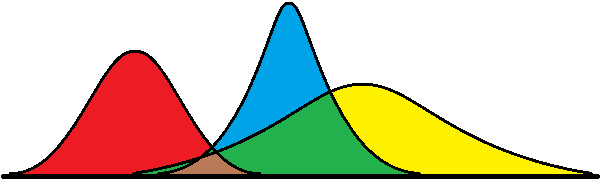
\includegraphics[width=.7\columnwidth]{GaussianDistOverlap1D.png}}
	}
\caption{A similarity index between three Gaussian distributions is illustrated as the summation of overlapping regions of two distributions (green) or three distributions (brown).
This concept is easily extended to multivariate Gaussian distributions.
}\label{fig:SimMeas}
\end{figure}

	
\subsection{Optimal Coalescence Avoidance}

%\EditTL{(Not sure we need this paragraph) Soft decision algorithms such as the JPDAF and M-JPDAF, which only consider estimate uncertainties when determining estimator gains, yield coalescence among the estimates. However, including a similarity index in an optimal fashion to determine each gain matrix serves to remove this coalescence.}

The proposed coalescence avoiding filtering algorithm is constructed by minimizing the cost function $\mathbf{J}\in\Re$, defined as as the sum of the uncertainty cost $J_P\in\Re$ and similarity cost $J_S\in\Re$ with positive weighting factor $c\in\Re$,
\begin{align}
\label{eqn:CostGen}
\mathbf{J}=J_P+cJ_S.
\end{align}
%The estimator gain $K_i$ is selected to minimize the above cost $\mathbf{J}$. In short, the estimator gain is chosen in the consideration of both uncertainty and coalescence, illustrated in Figure \ref{fig:CostTrends}.
The estimator gain $K_i$ is selected to minimize the above cost $\mathbf{J}$. By considering similarity to obtain the estimator gain, we mitigate some coalescence at the expense of increasing estimate uncertainty according to the magnitude of $c$.
The choice of $c$ depends on the type of scenario and the parameter $a$ shapes the similarity cost $J_S$.


\begin{figure}
\setlength{\unitlength}{0.06\columnwidth}
\centerline{\footnotesize\selectfont
\begin{picture}(8.5,7.3)(-0.5,-0.8)
\put(-0.5,3){\rotatebox{90}{Cost}}
\put(0,0){\includegraphics[width=0.48\columnwidth]{ECC14_fig1.pdf}}
\put(5.3,1.2){\shortstack[c]{Uncertainty\\ cost: $J_P$}}
\put(6.2,2.6){\shortstack[c]{Similarity\\ cost: $J_S$}}
\put(5.2,5.2){\shortstack[c]{Weighted sum:\\ $\mathbf{J}=J_P+cJ_S$}}
\put(4.98,0.78){\circle*{0.1}}
\put(2.48,1.57){\circle*{0.1}}
\put(4.8,-0.4){$K_{M-JPDAF}$}
\put(2.3,-0.4){$K_{C-JPDAF}$}
\put(3.1,-0.8){Estimator gain}
\end{picture}
}
\caption{Illustration of optimal coalescence avoidance: several costs are illustrated with respect to an element of an estimator gain $K$ (red: uncertainty cost $J_P$, blue: similarity cost $J_S$, black: weighted sum). The estimator gain $K_{M-JPDAF}$ is selected to minimize the uncertainty cost. The estimator gain $K_{C-JPDAF}$ is chosen such that the weighted sum of the uncertainty cost and the similarity cost is minimized. In short, at the expense of increased uncertainty at a single step, the proposed approach prevents coalescence. The increased uncertainty at each step is rewarded by reducing the overall estimation error drastically by maintaining correct data association during close proximity tracking scenarios or missions.}
\label{fig:CostTrends}
\end{figure}

\paragraph*{Uncertainty Cost}\ 
The uncertainty cost $J_P$ is defined as the sum of the trace of each posterior covariance as% the summation of \refeqn{JpIntro}:
\begin{align}
J_P=\sum\limits_{i}\tr{P^+_i},\label{eqn:JP}
\end{align}
where $P^+_{i}$ is obtained by \refeqn{JPDAFCov}, dependent on the gain $K_i$ at the current time step.
The derivative of $J_P$ is taken from \refeqn{Uncertainty0}
\begin{align}
\label{eqn:CostP}
\frac{\partial J_{P}}{\partial K_{i}}&=2K_iE_i-2(1-\beta_{0,i})P^-_iH_i^T.
\end{align}

\paragraph*{Similarity Cost}\ 
Any shared measurement $z_j$ on measurement estimate $\hat z_i$ yields an innovation $e_{ij}$ according to \refeqn{eij}.
During the measurement update, this innovation typically has the net effect of drawing $\hat z_i$ towards $z_j$ if $\beta_{ij}$ is nonzero.
This occurs for all estimates and all measurements; coalescence results when measurement estimates are drawn towards common measurements.
Therefore, coalescence of the JPDAF or M-JPDAF occurs inside the measurement space (e.g. if a sensor provides ranges and bearings, these are in the measurement space as opposed to a Cartesian state vector inside the state space).

Contrary to~\cite{KauLovLee14} where the similarity index is in terms of state space variables, the coalescence avoidance presented in this paper takes place inside the measurement space to most directly remove the coalescence.
Let the posterior measurement estimate be $\hat z_i^+\in\Re^m$, and define the innovation $e_{i}^+\in\Re^m$ as
\begin{align}
\hat z_i^+&=H_i\hat x_i^+,
\\
e_{i}^+&=z_i-\hat z_i^+=(H_ix_i+v_i)-H_i\hat x_{i}^+=H_i\tilde x_i^++v_i,
\end{align}
where $\tilde x_i^+=x_i-\hat x_{i}^+\in\Re^n$ denotes the error between the true state and the posterior estimate. The posterior innovation covariance $S^+_i\in\Re^{m\times m}$ is given by
\begin{align}
S^+_i=\mathrm{E}[e_i^+e_i^{+T}]=\mathrm{E}[(H_i\tilde x_i^++v_i)(H_i\tilde x_i^++v_i)^T]
=H_iP^+_iH_i^T+R_i.\label{eqn:Spi}
\end{align}
From these, the similarity cost $J_S$ is defined according to the format of \refeqn{zetaGeneral} as
%which are used to define $u_{p q}$ between $\hat z^+_{p}$ and $\hat z^+_{q}$:
\begin{align}
\label{eqn:Js}
J_S=\sum\limits_{\substack{p,q=1,\\p\neq q}}^{n_t}\exp (-au_{pq}),
\end{align}
where $u_{pq}\in\Re$ is a function of the innovation covariance summation $S^+_{pq}=S^+_{p}+S^+_{q}\in\Re^{m\times m}$,
\begin{align}
u_{pq} & = (\hat z_{p}^+-\hat z^+_{q})^T(S^+_{pq})^{-1}(\hat z^+_{p}-\hat z^+_{q})\label{eqn:U}.
\end{align}
%Expanding \refeqn{U} with respect to the $p$-th system,
Substituting the expression for $S_p^+$ obtained by \refeqn{Spi},
\begin{align}
u_{pq}=&\ 
(H_pK_p{\bar{e}}_p-\hat z^+_{q})^T
(H_pP^+_{p}H_p^T+R_p+S^+_q)^{-1}
(H_pK_p{\bar{e}}_p-\hat z^+_{q}).
\label{eqn:Up}
\end{align}

\begin{prop}
Let $b$, $d$, and $p$ be integers such that $b\in\{1,2,...,n\}$,  $d\in\{1,2,...,m\}$, and $p\in\{1,2,...,n_t\}$ such that the $(b,d)$-th element of the $p$-th gain matrix is written as $[K_p]_{bd}\in\Re$.
Also, let $\Ibd\in \Re^{n\times m}$ be defined such that its $(b,d)$-th element is one and other elements are zero.
Then the following partial derivative may be obtained,
\begin{align*}
\deriv{J_S}{[K_p]_{bd}}&=\ -a\sum\limits_{q,q\neq p}\exp (-au_{pq})
\{
2(H_p\Ibd{\bar{e}}_p)^T
{S_{pq}^+}^{-1}
\nonumber
\\
& \quad
-(H_pK_p{\bar{e}}_p-\hat z^+_{q})^T
{S^+_{pq}}^{-1}
H_p
[(1-\beta_{0,p})(\Ibd H_pP_p^-
+P_p^-H_p^T\Ibd^T)
\nonumber
\\
& \quad
-\Ibd E_pK_p^T-K_pE_p\Ibd^T]
H_p^T
{S^+_{pq}}^{-1}
\}(H_pK_p{\bar{e}}_p-\hat z^+_{q}).
%\\
%\mathcal{S}_{pq,p,bd}&=-{S^+_{pq}}^{-1}
%H_p
%[(1-\beta_{0,p})(\Ibd H_pP_p^-+P_p^-H_p^T\Ibd^T)-\Ibd E_pK_p^T\nonumber
%\\
%& \quad -K_pE_p\Ibd^T]
%H_p^T
%{S^+_{pq}}^{-1}.
\end{align*}
\end{prop}
\begin{proof}
See the Appendix B.
\end{proof}


Necessary conditions for optimality are given by
\begin{align}
\deriv{\mathbf{J}}{K_i} = \deriv{J_P}{K_i} + c \deriv{J_S}{K_i} =0,\label{eqn:NCO}
\end{align}
where $\deriv{J_P}{K_i}$ and $\deriv{J_S}{K_i}$ may be nonzero, so the result may be different than \refeqn{GainK}, which only considers state estimate uncertainty in the optimization.
In short, \refeqn{CostP} and \refeqn{JSK} are substituted into \refeqn{NCO} and repeated for all $p$ to obtain $n_t$ optimal gain matrices.
Then, the C-JPDAF is completed by updating the state estimate and covariance by using \refeqn{KalEst} and \refeqn{JPDAFCov}, respectively.


As the optimality condition is a nonlinear function of estimator gains, there is no closed-form solution.
Hence, we require a nonlinear equation solver.
When $c=0$, we can show that the optimal gain reduces to that of the M-JPDAF, which is used as an initial guess during iterative numerical methods.
%Therefore, if the number of estimates exhibiting significant similarity is $n_t^*\leq n_t$ and $\mathcal C$ is the number of times \refeqn{NCO} is solved depending on the numerical accuracy, then the required iterations is $n_t^*(n_t^*-1)\mathcal C$, where some variables may be reused (e.g. $S^+_{pq}\equiv S^+_{qp}$) and often the effect of \refeqn{derivu} is negligible with large estimate separations.





\section{Numerical Examples}
\label{sec:NE}

We consider satellites in the low earth orbit (LEO) and in the geosynchronous orbit (GEO) to compare the performances of the conventional JPDAF, the M-JPDAF, and the C-JPDAF.
The satellites are subject to the dynamics of the two-body problem.
Since the system dynamics $\dot x=f(x)$ is nonlinear, the linearized matrix $F_{i_{k-1}}=\deriv{f}{x_i}\bigg|_{x_i=\hat x_{i_{k-1}}^+}$ is used with \refeqn{xestapriori} and \refeqn{Papriori}.
Similarly, the measurement dynamics $z_i = h(x_i)$ may experience nonlinearities (e.g. range, range rate, bearing), the linearized matrix $H_i=\deriv{h_i}{x_i}\bigg|_{x_i=\hat x_{i}^-}$ is used with \refeqn{GainK}, \refeqn{JPDAFPostCovSimpleUpdate}, \refeqn{CostP}, \refeqn{Spi}, and \refeqn{Up}.

Let $\vec r=\begin{bmatrix}x_1, & x_2, & x_3\end{bmatrix}^T\in\Re^3$ be the position vector of the $i$-th satellite represented with respect to the Earth-Centered Inertial (ECI) frame.
The equation of motion corresponding to the two-body problem is given by
\begin{align}
\label{eqn:NonLin2BP}
\ddot{\vec r}&=-\frac{\mu}{r^3}\vec r=-\mu(\vec r^T\vec r)^{-\frac32}\vec r,
\end{align}
where $\mu=398,600\ \frac{km^3}{sec^2}$ is the gravitational constant of the earth if position is estimated in kilometers and time is measured in seconds~\cite{Val01}.

Let $\delta$ denote an infinitesimal change of a state variable.
The linearized equations of state variable $\vec x=\begin{bmatrix}\vec r^T, & \dot{\vec r}^T\end{bmatrix}^T\in\Re^6$ are based on \refeqn{NonLin2BP} and given by
\begin{align}
\begin{bmatrix}
\delta\dot{\vec r} \\ \delta\ddot{\vec r}
\end{bmatrix}
%\delta\dot{\vec x}
=
\begin{bmatrix}
0_{3\times3}, & I_{3\times3} \\
\mu\left[3\vec r({\vec r}^T\vec r)^{-\frac52}{\vec r}^T-({\vec r}^T\vec r)^{-\frac32}I_{3\times3}\right], & 0_{3\times3}
\end{bmatrix}
\begin{bmatrix}
\delta\vec r \\ \delta\dot{\vec r}
\end{bmatrix}
%\delta\vec x
.
\end{align}
%Defining the above square matrix as $A_{lin}$, the linearized state transition matrix over the time step $dt$ is defined as
%\begin{align}
%F=\expm{(A_{lin}dt)}
%\end{align}
%where $\expm$ denotes the matrix exponential function.

The process uncertainty may be subject to a variety of perturbations beyond two-body forces; in the following simulations, let these uncertainties be summarized with the standard deviation of position $\sigma_r\in\Re$ and velocity $\sigma_{\dot r}\in\Re$ such that the process covariance is defined as $Q=\diag[\sigma_r^2I_{3\times3}, \sigma_{\dot r}^2I_{3\times3}]\in\Re^{6\times6}$, where $\sigma_r$ and $\sigma_{\dot r}$ take several values depending on the case considered.
%=\diag[10^{-6}I_{3\times3}, 10^{-8}I_{3\times3}]$.

For all cases, the satellites are measured with a phased-array radar (LEO) or telescope (GEO) at the location $\vec r_s\in\Re^3$ on the equator in the ECI frame, which has nonzero velocity due to the rotation of the earth,
\begin{align}
\vec r_s=R_E
\begin{bmatrix}
\cos\frac{2\pi t}T, & \sin\frac{2\pi t}T, & 0
\end{bmatrix}^T,
\quad
\dot{\vec r}_s=\frac{2\pi tR_E}T
\begin{bmatrix}
-\sin\frac{2\pi t}T,  & \cos\frac{2\pi t}T, & 0
\end{bmatrix}^T,
\end{align}
where $R_E=6378$ km is the radius of the earth, time of the day $t$ starts at $0$ seconds, and the time period of the day is $T=86164.090518$ seconds.
Here, the measurements consist of the range $\rho$ between the sensor and the satellite (km), the range rate $\dot\rho$ (km/sec), and topocentric right ascension $\alpha$ and declination $\delta$ (rad)~\cite{Val01}, i.e., the $j$-th measurement $z_j$ ($z_j\in\Re^4$ in LEO and $z_j\in\Re^2$ in GEO) is
\begin{align}
\label{eqn:zj}
z_j=\begin{cases}
                        \begin{bmatrix}\rho, & \dot\rho, & \alpha, & \delta\end{bmatrix}^T \text{for LEO satellites} \\
                        \begin{bmatrix}\alpha, & \delta\end{bmatrix}^T \qquad\  \text{for GEO satellites}
                    \end{cases}
.
\end{align}
%The standard deviations $\sigma_\rho$, $\sigma_\alpha$, and $\sigma_\delta$ are based on the Mahe Ground Station uncertainty data~\cite{VerSauSco04} and $\sigma_{\dot\rho}$ from the examples from~\cite{KurAriAriEfe10}.


%For each following scenario, several cases are simulated where various parameters are slightly changed with $\epsilon\in\Re$, summarized in Table \ref{tab:CaseDef}, and measurement are simulated with \refeqn{NonLin2BP} and \refeqn{zj}.
In the following scenarios, several cases are simulated with \refeqn{NonLin2BP} and measurements are generated according to \refeqn{zj}.
For all cases and time steps, measurements may originate from satellites, but this origin is not given to the data association algorithm.
Additionally, there is a $10\%$ chance that a measurement is either deleted or an extraneous measurement is added at each time step.
Further descriptions of the cases are available below, and the resulting accuracy is measured with RMS error, the uncertainty is summarized with $\tr{J_P}$, and the computation time is measured as well, tabulated in Tables \ref{tab:A1}--\ref{tab:B2}.
Scenarios A1 and B1 are data association and filtering examples in LEO, while scenarios A2 and B2 are GEO examples.
For readers with interest in how the algorithms handle perturbations, various parameters are slightly changed with $\epsilon\in\Re$, summarized in Table \ref{tab:CaseDef}.
The metrics from the perturbed cases are summarized in the subsequent tables as well.


\begin{table}
\begin{center}
\caption{Case Definitions} \label{tab:CaseDef}
\begin{threeparttable}[h]
\begin{tabularx}{.65\textwidth}
{
>{$}c<{$} |
>{$}c<{$}
}
\toprule
\multirow{2}{*}{Symbol} & \multirow{2}{*}{Explanation}\\
\\
\midrule
\multirow{1}{*}{A} &  \multirow{1}{*}{Comparison of JPDAF and M-JPDAF}
\\
\multirow{1}{*}{B} &  \multirow{1}{*}{Comparison of JPDAF, M-JPDAF, and C-JPDAF}
\\
\multirow{1}{*}{1} &  \multirow{1}{*}{Orbits in LEO}
\\
\multirow{1}{*}{2} &  \multirow{1}{*}{Orbits in GEO}
\\
\multirow{1}{*}{a} &  \multirow{1}{*}{$\sigma^2_{\rho,a} = \epsilon\sigma^2_{\rho}$}
\\
\multirow{1}{*}{b} &  \multirow{1}{*}{$\sigma^2_{\dot \rho,b} = \epsilon\sigma^2_{\dot \rho}$}
\\
\multirow{1}{*}{c} &  \multirow{1}{*}{$\sigma^2_{\rho,c} = \epsilon\sigma^2_{\rho}$, $\sigma^2_{\dot \rho,c} = \epsilon\sigma^2_{\dot \rho}$}
\\
\multirow{1}{*}{d} &  \multirow{1}{*}{$\sigma^2_{\alpha,d} = \epsilon\sigma^2_{\alpha}$, $\sigma^2_{\delta,d} = \epsilon\sigma^2_{\delta}$}
\\
\multirow{1}{*}{e} &  \multirow{1}{*}{$\sigma^2_{\mathbf{\rho},e} = \epsilon\sigma^2_{\mathbf{\rho}}$ (scenario 1 only)}
\\
\multirow{1}{*}{f} &  \multirow{1}{*}{$\sigma^2_{\mathbf{\dot\rho},f} = \epsilon\sigma^2_{\mathbf{\dot\rho}}$ (scenario 1 only)}
\\
\bottomrule
\end{tabularx}
\end{threeparttable}
\end{center}
\end{table}

\subsection{Data Association and Filtering in LEO}

Various cases in LEO are simulated to compare the data association and filtering algorithms, namely the JPDAF, M-JPDAF, and C-JPDAF.
The measurement uncertainty is $R=\diag[\sigma_\rho^2, \sigma_{\dot\rho}^2, \sigma_\alpha^2, \sigma_\delta^2]=\\\diag[(0.15\ \text{km})^2, (0.005\ \text{km/s})^2, (\frac{0.01\pi}{180}\ \text{rad})^2, (\frac{0.01\pi}{180}\ \text{rad})^2]\in\Re^{4\times4}$ where these standard deviations are selected from the Mahe Ground Station uncertainty data~\cite{VerSauSco04} and ~\cite{KurAriAriEfe10}.

\paragraph*{Scenario A1: Comparison of the JPDAF and M-JPDAF with two LEO satellites in close proximity}\ 

The first set of cases compares the JPDAF with the M-JPDAF for tracking two nearby satellites passing over the sensor field of view in LEO. The initial conditions of the first two orbits are chosen as
\begin{align}
x_{1,A1}&=x_{ref,A1}+x_{pert,A1}, \quad x_{2,A1}=x_{ref,A1}-x_{pert,A1},\nonumber
\\
x_{ref,A1}&=\begin{bmatrix}7000\ \text{km}, & 0\ \text{km}, & 1000\ \text{km}, & 0\ \text{km/s}, & 7.546\ \text{km/s}, & 0\ \text{km/s}\end{bmatrix}^T,
\nonumber\\
x_{pert,A1}&=\begin{bmatrix}
0.2\ \text{km}, & 0\ \text{km}, & 0\ \text{km}, & 0\ \text{km/s}, & -0.105\ \text{km/s}, & 0\ \text{km/s}
\end{bmatrix}^T.\nonumber
\end{align}
In these cases, the process covariance is $Q=\diag[10^{-6}I_{3\times3}\ \text{km}^2, 10^{-8}I_{3\times3}\ \text{km/s}^2]$, the estimates have initial covariances matrix $P_{0,A1}=10^7\times Q$, time steps of $1$ second over $100$ seconds, and $\epsilon=10$ for the perturbed cases.
These scenarios are chosen because the estimates exhibit large initial uncertainties, so the spread in the innovations term from \refeqn{tildeP} affects the updates.
The gain of the M-JPDAF accounts for this portion of the state covariance matrix better than the gain for the conventional JPDAF in every single case.

Given identical parameters and measurements, the RMS errors of the position and the mean uncertainty cost $J_P$ defined in \refeqn{JP} are lower in \emph{every} case when the M-JPDAF is applied compared with when the conventional JPDAF is applied.
%In fact in two cases, namely A1b and A1c, the JPDAF is incapable of decreasing the estimate uncertainty as quickly as the M-JPDAF.
In two cases, namely A1b and A1c, the JPDAF suffers from track swapping, which is when measurements are consistently associated incorrectly.
%; the JPDAF initially suffers from such great coalescence that the estimates become associated with incorrect measurements consistently, known as track swapping.
Furthermore, the computational time is roughly the same between the JPDAF and M-JPDAF, so the results suggest that the improvement in accuracy is at no increase in computation.
These results are tabulated in Table \ref{tab:A1}, and some cases are plotted in Figure \ref{fig:A1}.


\begin{center}
\begin{threeparttable}[h]
\caption{Cases of A1} \label{tab:A1}
\begin{tabularx}{\textwidth}
{
>{$}c<{$} |
*{2}{>{$}c<{$}} |
*{2}{>{$}c<{$}} |
*{2}{>{$}c<{$}}
}
\toprule
\multirow{2}{*}{Case} & \multicolumn{2}{c}{\multirow{1}{*}{RMS Position Err. (km)}} & \multicolumn{2}{c}{\multirow{1}{*}{Time (sec)}} & \multicolumn{2}{c}{\multirow{1}{*}{Mean $J_P$}} \\
 & \multirow{1}{*}{JPDAF} & \multirow{1}{*}{M-JPDAF} & \multirow{1}{*}{JPDAF} & \multirow{1}{*}{M-JPDAF} & \multirow{1}{*}{JPDAF} & \multirow{1}{*}{M-JPDAF}
\\
\midrule
\text{A1}  & 0.12026 & 0.10646 & 0.582 & 0.561 & 0.5125 & 0.49054 \\
\text{A1a} & 0.17910 & 0.17157 & 0.558 & 0.561 & 4.6154 & 4.5607 \\
\text{A1b} & \hilight{2.63710} & 0.14150 & 0.562 & 0.559 & 1.9718 & 0.68328 \\
\text{A1c} & \hilight{2.63520} & 0.19559 & 0.570 & 0.579 & 5.7223 & 4.8463 \\
\text{A1d} & 0.20204 & 0.18865 & 0.573 & 0.578 & 0.59901 & 0.57227 \\
\text{A1e} & 0.14541 & 0.13361 & 0.576 & 0.574 & 0.53064 & 0.50884 \\
\text{A1f} & 0.12175 & 0.10795 & 0.576 & 0.560 & 0.51338 & 0.49086 \\
\bottomrule
\end{tabularx}
{\small
\begin{tablenotes}
    \item \hilight{Track swapping occurs}
  \end{tablenotes}}
\end{threeparttable}
\end{center}


\begin{figure}
{
%\hspace*{0.05\columnwidth}
\centerline{
	\subfigure[\;Case A1: JPDAF]
		{\hspace*{0.\columnwidth}\includegraphics[width=0.5\columnwidth]{A1JPDAF.pdf}}
	\subfigure[\;Case A1: M-JPDAF]
		{\hspace*{0.\columnwidth}\includegraphics[width=0.5\columnwidth]{A1MUJPDAF.pdf}}
	}
\centerline{
	\subfigure[\;Case A1b: JPDAF]
		{\hspace*{0.\columnwidth}\includegraphics[width=0.5\columnwidth]{A1bJPDAF.pdf}}
	\subfigure[\;Case A1b: M-JPDAF]
		{\hspace*{0.\columnwidth}\includegraphics[width=0.5\columnwidth]{A1bMUJPDAF.pdf}}
	}
\centerline{
	\subfigure[\;Case A1d: JPDAF]
		{\hspace*{0.\columnwidth}\includegraphics[width=0.5\columnwidth]{A1dJPDAF.pdf}}
	\subfigure[\;Case A1d: M-JPDAF]
		{\hspace*{0.\columnwidth}\includegraphics[width=0.5\columnwidth]{A1dMUJPDAF.pdf}}
	}
}
\caption{The orbital radii of three cases are shown where the dashed plots are the true trajectories and the solid plots are the estimated trajectories.
In all of these cases, the M-JPDAF is more accurate and avoids track swapping (Case A1b in particular).
% experiences less coalescence than the JPDAF.
%In particular, when the JPDAF is used in Case A1b, the initial coalescence causes track swapping.
Additionally, Case A1d experiences the most inaccurate estimation without track swapping with very noisy angle measurements, and the M-JPDAF has lower RMS error when compared to the JPDAF.
}\label{fig:A1}
\end{figure}

\paragraph*{Scenario B1: Comparison of the JPDAF, M-JPDAF, and C-JPDAF with three LEO satellites in close proximity}\ 

The JPDAF, M-JPDAF, and C-JPDAF algorithms are compared for three satellites in LEO with initial conditions
\begin{align}
x_{1,B1}&=x_{ref,B1}+x_{pert,B1}, \quad x_{2,B1}=x_{ref,B1}-x_{pert,B1}, \quad x_{3,B1}=x_{ref,B1},\nonumber
\\
x_{ref,B1}&=\begin{bmatrix}7000\ \text{km}, & 0\ \text{km}, & 0\ \text{km}, & 0\ \text{km/s}, & 7.546\ \text{km/s}, & 0\ \text{km/s}\end{bmatrix}^T,
\nonumber\\
x_{pert,B1}&=\begin{bmatrix}
0.025\ \text{km}, & 0\ \text{km}, & 0\ \text{km}, & 0\ \text{km/s}, & 0\ \text{km/s}, & 0\ \text{km/s}
\end{bmatrix}^T,\nonumber
\end{align}
where $Q=\diag[10^{-6}I_{3\times3}\ \text{km}^2, 10^{-8}I_{3\times3}\ \text{km/s}^2]$, $P_{0,B1}=Q$, and $\epsilon=1.1$ for time steps of $10$ seconds over a $2000$ second time period.
This corresponds to a phased-array radar observing a slow separation of LEO objects in a near-circular orbit; because the satellite states are in close proximity over a large time period, the JPDAF and M-JPDAF are subject to severe coalescence.
The C-JPDAF is designed to avoid this coalescence, where the parameters $a=5\times10^{-1}$ and $c=2.3\times10^{-4}$ from \refeqn{zetaGeneral} and \refeqn{CostGen} are used in these scenarios from trial and error.
The accuracy of the C-JPDAF is largely improved from that of the JPDAF and M-JPDAF; however, the computational cost of the C-JPDAF is roughly $60$ times that of either other algorithm.
The position RMS errors and computation times are tabulated in Table \ref{tab:B1} and example plots from these cases are shown in Figure \ref{fig:B1}.

\begin{center}
\begin{threeparttable}[h]
\caption{Case B1} \label{tab:B1}
\begin{tabularx}{\textwidth}
{
>{$}c<{$} |
*{3}{>{$}c<{$}} |
*{3}{>{$}c<{$}}
}
\toprule
\multirow{2}{*}{Case} & \multicolumn{3}{c}{\multirow{1}{*}{RMS Position Err. (km)}} & \multicolumn{3}{c}{\multirow{1}{*}{Time (sec)}} \\
 & \multirow{1}{*}{JPDAF} & \multirow{1}{*}{M-JPDAF} & \multirow{1}{*}{C-JPDAF} & \multirow{1}{*}{JPDAF} & \multirow{1}{*}{M-JPDAF} & \multirow{1}{*}{C-JPDAF}
\\
\midrule
\text{B1}   	& 0.14432 & 0.091133 & 0.057312 & 1.74 & 1.67 & 101 \\
\text{B1a} 	& 0.14432 & 0.091134 & 0.057307 & 1.69 & 1.73 & 101 \\
\text{B1b} 	& 0.14694 & 0.094506 & 0.055145 & 1.67 & 1.68 & 101 \\
\text{B1c} 	& 0.14693 & 0.094507 & 0.055136 & 1.68 & 1.67 & 101 \\
\text{B1d} 	& 0.14400 & 0.088933 & 0.058911 & 1.66 & 1.66 & 103 \\
\text{B1e} 	& 0.14408 & 0.090823 & 0.059919 & 1.67 & 1.67 & 100 \\
\text{B1f} 	& 0.14436 & 0.091212 & 0.064299 & 1.73 & 1.72 & 98.7 \\
\bottomrule
\end{tabularx}
\begin{tabularx}{.52\textwidth}
{
>{$}c<{$} |
*{3}{>{$}c<{$}}
}
\multirow{2}{*}{Case} & \multicolumn{3}{c}{\multirow{1}{*}{Mean $J_P$}} \\
 & \multirow{1}{*}{JPDAF} & \multirow{1}{*}{M-JPDAF} & \multirow{1}{*}{C-JPDAF}
\\
\midrule
\text{B1}   	    	& 0.24559 & 0.17819 & 0.17958 \\
\text{B1a} 		& 0.24559 & 0.17819 & 0.17959 \\
\text{B1b} 		& 0.25349 & 0.18386 & 0.18510 \\
\text{B1c} 		& 0.25350 & 0.18386 & 0.18511 \\
\text{B1d} 		& 0.26058 & 0.18944 & 0.19177 \\
\text{B1e} 		& 0.24626 & 0.17861 & 0.1794 \\
\text{B1f} 		& 0.24561 & 0.17820 & 0.18009\\
\bottomrule
\end{tabularx}
\end{threeparttable}
\end{center}

\begin{figure}
{
%\hspace*{0.05\columnwidth}
\centerline{
	\subfigure[\;Case B1: JPDAF]
		{\hspace*{0.\columnwidth}\includegraphics[width=0.33\columnwidth]{B1JPDAF.pdf}}
	\subfigure[\;Case B1: M-JPDAF]
		{\hspace*{0.\columnwidth}\includegraphics[width=0.33\columnwidth]{B1MUJPDAF.pdf}}
	\subfigure[\;Case B1: C-JPDAF]
		{\hspace*{0.\columnwidth}\includegraphics[width=0.33\columnwidth]{B1C-JPDAF.pdf}}
	}
\centerline{
	\subfigure[\;Case B1c: JPDAF]
		{\hspace*{0.\columnwidth}\includegraphics[width=0.33\columnwidth]{B1cJPDAF.pdf}}
	\subfigure[\;Case B1c: M-JPDAF]
		{\hspace*{0.\columnwidth}\includegraphics[width=0.33\columnwidth]{B1cMUJPDAF.pdf}}
	\subfigure[\;Case B1c: C-JPDAF]
		{\hspace*{0.\columnwidth}\includegraphics[width=0.33\columnwidth]{B1cC-JPDAF.pdf}}
	}
\centerline{
	\subfigure[\;Case B1f: JPDAF]
		{\hspace*{0.\columnwidth}\includegraphics[width=0.33\columnwidth]{B1fJPDAF.pdf}}
	\subfigure[\;Case B1f: M-JPDAF]
		{\hspace*{0.\columnwidth}\includegraphics[width=0.33\columnwidth]{B1fMUJPDAF.pdf}}
	\subfigure[\;Case B1f: C-JPDAF]
		{\hspace*{0.\columnwidth}\includegraphics[width=0.33\columnwidth]{B1fC-JPDAF.pdf}}
	}
}
\caption{The orbital radii of three cases are shown where the dashed plots are the true trajectories and the solid plots are the estimated trajectories.
In all cases the M-JPDAF is more accurate and experiences less coalescence than the JPDAF, but both algorithms suffer from coalescence.
The C-JPDAF systematically removes this coalescence from the updates at the cost of covariance matrices with slightly larger traces and a large increase in required computational resources.
%Between Cases B1 and B1c, the process position uncertainty is increased, which last little effect on the estimates since this has little
The conditions that affect the C-JPDAF most are with Case B1f where the range-rate measurements have the greatest uncertainty.
}\label{fig:B1}
\end{figure}

Among the variations of the B1 cases, the range-rate measurement uncertainty (Case B1f) has the largest effect on tracking with the C-JPDAF.
The velocities of satellites in LEO are very large, so a small increase in $\sigma_{\dot\rho}$ corresponds to a large decrease in $J_S$, i.e., the measurement sets for the satellites will be less similar.  This is further shown with the smallest computational cost among the B1 cases.
Hence, the similarity optimization is very sensitive to velocity measurement uncertainty in these cases.
%This can be explained because in the B1 cases, the ranges and bearings of each track are close and changing, but the difference between the velocities of the three satellites remain largely constant after about $500$ seconds.
%As long as the estimates are able to stay sufficiently far apart, as the C-JPDAF is able to accomplish, the component of the velocity measurement in the radial direction serves as a distinguishing portion of the full measurement, so that the correct association between measurement and estimate is more heavily weighted, and hence better tracking is achieved.
%The quality of the range-rate measurement is degraded in Case B1f, and hence the C-JPDAF algorithm is not able to as accurately track each estimate when compared with the other B1 cases.




















\subsection{Data Association and Filtering in GEO}

The data association and filtering algorithms are simulated in various GEO scenarios.
Angles-only measurements are available with higher accuracy; namely the topocentric right ascension and declination are chosen as $\sigma_{\alpha,GEO}=\sigma_{\delta,GEO}=10^{-2}\sigma_\alpha$ and the $j$-th measurement $z_{j,GEO}\in\begin{bmatrix}\alpha, & \delta\end{bmatrix}^T\in\Re^2$ with covariance $R=\diag[\sigma_{\alpha,GEO}^2, \sigma_{GEO,\delta}^2]\in\Re^{2\times2}$.% YOU MAY HAVE TO REMOVE "\\" WITH ANY EDITING CHANGES













\paragraph*{Scenario A2: Comparison of the JPDAF and M-JPDAF with two near-GEO satellites in close proximity}\ 

These cases serve to compare the JPDAF with the M-JPDAF for tracking two nearby satellites passing over the sensor field of view in GEO, where the orbital radius is $r_{GEO}=4.2164\times10^{4}\ \text{km}$. The initial conditions of the first two orbits are chosen as
\begin{align*}
x_{1,A2}&=\begin{bmatrix}r_{GEO}, & 0\ \text{km}, & 0\ \text{km}, & 0\ \text{km/s}, & \sqrt{\frac{\mu}{r_{GEO}}}, & 0\ \text{km/s}\end{bmatrix}^T,
\\
x_{2,A2}&=x_{1,A2}+\begin{bmatrix}
0\ \text{km}, & 0\ \text{km}, & -1\ \text{km}, & 0\ \text{km/s}, & 0\ \text{km/s}, & 4\times10^{-4}\ \text{km/s}
\end{bmatrix}^T,
\end{align*}
or where $x_{1,A2}$ remains exactly in GEO while $x_{2,A2}$ starts slightly perturbed from a GEO orbit with a nonzero inclination such that the two satellites nearly collide as they pass by in close proximity.
The A2 cases consider small initial covariance matrices $P_{0,A2}= Q$ where $Q=\diag[10^{-6}I_{3\times3}, 10^{-8}I_{3\times3}]$, time steps of $10$ seconds over $5000$ seconds, and $\epsilon=1.1$.
%These scenarios are chosen because the estimates exhibit large initial uncertainties, so the spread in the innovations affects the updates.
Even though the initial conditions are largely different from those of the A1 cases, the A2 cases display the same trends, where the computational costs among the algorithms are roughly the same but the tracking abilities of the M-JPDAF \emph{always} yield estimates closer to the truth with less uncertainty than those of the JPDAF.
These results are tabulated in Table \ref{tab:A2}, and some cases are plotted in Figure \ref{fig:A2}.

\begin{center}
\begin{threeparttable}[h]
\caption{Case A2} \label{tab:A2}
\begin{tabularx}{\textwidth}
{
>{$}c<{$} |
*{2}{>{$}c<{$}} |
*{2}{>{$}c<{$}} |
*{2}{>{$}c<{$}}
}
\toprule
\multirow{2}{*}{Case} & \multicolumn{2}{c}{\multirow{1}{*}{RMS Angular Err. ($10^{-6}$rad)}} & \multicolumn{2}{c}{\multirow{1}{*}{Time (sec)}} & \multicolumn{2}{c}{\multirow{1}{*}{Mean $J_P$}} \\
 & \multirow{1}{*}{JPDAF} & \multirow{1}{*}{M-JPDAF} & \multirow{1}{*}{JPDAF} & \multirow{1}{*}{M-JPDAF} & \multirow{1}{*}{JPDAF} & \multirow{1}{*}{M-JPDAF}
\\
\midrule
\text{A2}  & 1.2140 & 0.98784 & 2.77 & 2.73 & 16.5052 & 16.5015 \\
\text{A2a} & 1.2141 & 0.98780 & 2.74 & 2.74 & 16.5054 & 16.5017 \\
\text{A2b} & \hilight{11.728} & 1.0143 & 2.73 & 2.74 & 18.1526 & 18.1477 \\
\text{A2c} & \hilight{11.728} & 1.0142 & 2.73 & 2.75 & 18.1528 & 18.1479 \\
\text{A2d} & \hilight{11.700} & 1.0332 & 2.82 & 2.77 & 16.511 & 16.5054 \\
\bottomrule
\end{tabularx}
{\small
\begin{tablenotes}
    \item \hilight{Track swapping occurs}
  \end{tablenotes}}
\end{threeparttable}
\end{center}

\begin{figure}
{
%\hspace*{0.05\columnwidth}
\centerline{
	\subfigure[\;Case A2: JPDAF]
		{\hspace*{0.\columnwidth}\includegraphics[width=0.5\columnwidth]{A2JPDAF.pdf}}
	\subfigure[\;Case A2: M-JPDAF]
		{\hspace*{0.\columnwidth}\includegraphics[width=0.5\columnwidth]{A2MUJPDAF.pdf}}
	}
\centerline{
	\subfigure[\;Case A2a: JPDAF]
		{\hspace*{0.\columnwidth}\includegraphics[width=0.5\columnwidth]{A2aJPDAF.pdf}}
	\subfigure[\;Case A2a: M-JPDAF]
		{\hspace*{0.\columnwidth}\includegraphics[width=0.5\columnwidth]{A2aMUJPDAF.pdf}}
	}
\centerline{
	\subfigure[\;Case A2b: JPDAF]
		{\hspace*{0.\columnwidth}\includegraphics[width=0.5\columnwidth]{A2bJPDAF.pdf}}
	\subfigure[\;Case A2b: M-JPDAF]
		{\hspace*{0.\columnwidth}\includegraphics[width=0.5\columnwidth]{A2bMUJPDAF.pdf}}
	}
}
\caption{The orbital radii of three cases are shown where the dashed plots are the true trajectories and the solid plots are the estimated trajectories and $\alpha_{diff}$ is the difference between $\alpha_{1}$ and the measurement estimates of the two tracks.
Cases A2 and A2a serve as examples where the coalescence during crossing periods with the JPDAF yields much more similar estimates than with the M-JPDAF.
In Case A2b, this coalescence is so severe that track swapping occurs with the JPDAF, but this is avoided with the M-JPDAF.
}\label{fig:A2}
\end{figure}








































\paragraph*{Scenario B2: Comparison of the JPDAF, M-JPDAF, and C-JPDAF with two GEO satellites in close proximity}\ 

The JPDAF, M-JPDAF, and C-JPDAF algorithms are compared for two satellites in GEO with initial conditions
\begin{align}
\begin{split}
x_{1,B2}&=f_{GEO}(0^\circ), \quad x_{2,B2}=f_{GEO}({10^{-4}}^\circ), \quad \mbox{where}
\\
f_{GEO}(\theta)&=r_{GEO}\begin{bmatrix}\cos\theta, & \sin\theta, & 0, & -\sqrt{\frac{\mu}{r_{GEO}^3}}\sin\theta, & \sqrt{\frac{\mu}{r_{GEO}^3}}\cos\theta, & 0\end{bmatrix}^T,
\end{split}
\end{align}
where $Q=\diag[10^{-8}I_{3\times3}\ \text{km}^2, 10^{-10}I_{3\times3}\ \text{km/s}^2]$, $P_{0,B}=Q$, and $\epsilon=1.1$ for time steps of $10$ seconds over a $2000$ second time period.
This corresponds to a scenario where two satellites orbit steadily nearby in GEO.
For the C-JPDAF, the parameters $a=1.5\times10^{2}$ and $c=1\times10^{10}$ from \refeqn{zetaGeneral} and \refeqn{CostGen} are used in these scenarios from trial and error.
In theory, topocentric right ascension measurements should be the same distance apart throughout the cases and the declination should always be zero.
Much like the B1 cases, the accuracy of the C-JPDAF yields a large improvement from that of the JPDAF and M-JPDAF; however, the increase in computational cost of the C-JPDAF is roughly $30$ times that of either other algorithm, which is about half of the increase found with the B1 cases.
This is because the similarity measure is less complex with the B2 cases than with the B1 cases due to the number of estimates and the size of the measurement space.
The angular RMS errors and computation times are tabulated in Table \ref{tab:B2} and some example plots from these cases are shown in Figure \ref{fig:B2}. In applications with a large number of objects to track, the C-JPDAF need not be applied on most objects; only those close neighbors where the similarity among the estimates yield coalescence with the JPDAF or the M-JPDAF. This way, a data association scheme with an analytic solution, such as the JPDAF or the M-JPDAF, could be applied to the remaining estimates to mitigate the large computational requirements of the C-JPDAF.





\begin{center}
\begin{threeparttable}[h]
\caption{Case B2} \label{tab:B2}
\begin{tabularx}{0.98\textwidth}
{
>{$}c<{$} |
*{3}{>{$}c<{$}} |
*{3}{>{$}c<{$}}
}
\toprule
\multirow{2}{*}{Case} & \multicolumn{3}{c}{\multirow{1}{*}{RMS Angular Err. ($10^{-6}$rad)}} & \multicolumn{3}{c}{\multirow{1}{*}{Time (sec)}} \\
 & \multirow{1}{*}{JPDAF} & \multirow{1}{*}{M-JPDAF} & \multirow{1}{*}{C-JPDAF} & \multirow{1}{*}{JPDAF} & \multirow{1}{*}{M-JPDAF} & \multirow{1}{*}{C-JPDAF}
\\
\midrule
\text{B2}   	& 1.111 & 0.9478 & 0.5671 & 1.15 & 1.12 & 34.3 \\
\text{B2a} 	& 1.111 & 0.9478 & 0.5635 & 1.15 & 1.15 & 34.8 \\
\text{B2b} 	& 1.131 & 0.9829 & 0.5739 & 1.13 & 1.13 & 35.3 \\
\text{B2c} 	& 1.131 & 0.9829 & 0.5644 & 1.12 & 1.13 & 34.8 \\
\text{B2d} 	& 1.112 & 0.9544 & 0.5614 & 1.11 & 1.12 & 35.2 \\
\bottomrule
\end{tabularx}
\begin{tabularx}{.57\textwidth}
{
>{$}c<{$} |
*{3}{>{$}c<{$}}
}
\multirow{2}{*}{Case} & \multicolumn{3}{c}{\multirow{1}{*}{Mean $J_P$}} \\
 & \multirow{1}{*}{JPDAF} & \multirow{1}{*}{M-JPDAF} & \multirow{1}{*}{C-JPDAF}
\\
\midrule
\text{B2}   	    	& 0.0076169 & 0.0073684 & 0.0073846 \\
\text{B2a} 		& 0.007617 & 0.0073685 & 0.0073879 \\
\text{B2b} 		& 0.0083158 & 0.0080603 & 0.0080799 \\
\text{B2c} 		& 0.0083159 & 0.0080604 & 0.0080812 \\
\text{B2d} 		& 0.0076643 & 0.0074103 & 0.0074331 \\
\bottomrule
\end{tabularx}
\end{threeparttable}
\end{center}

\begin{figure}
{
%\hspace*{0.05\columnwidth}
\centerline{
	\subfigure[\;Case B2: JPDAF]
		{\hspace*{0.\columnwidth}\includegraphics[width=0.33\columnwidth]{B2JPDAF.pdf}}
	\subfigure[\;Case B2: M-JPDAF]
		{\hspace*{0.\columnwidth}\includegraphics[width=0.33\columnwidth]{B2MUJPDAF.pdf}}
	\subfigure[\;Case B2: C-JPDAF]
		{\hspace*{0.\columnwidth}\includegraphics[width=0.33\columnwidth]{B2C-JPDAF.pdf}}
	}
\centerline{
	\subfigure[\;Case B2b: JPDAF]
		{\hspace*{0.\columnwidth}\includegraphics[width=0.33\columnwidth]{B2bJPDAF.pdf}}
	\subfigure[\;Case B2b: M-JPDAF]
		{\hspace*{0.\columnwidth}\includegraphics[width=0.33\columnwidth]{B2bMUJPDAF.pdf}}
	\subfigure[\;Case B2b: C-JPDAF]
		{\hspace*{0.\columnwidth}\includegraphics[width=0.33\columnwidth]{B2bC-JPDAF.pdf}}
	}
\centerline{
	\subfigure[\;Case B2d: JPDAF]
		{\hspace*{0.\columnwidth}\includegraphics[width=0.33\columnwidth]{B2dJPDAF.pdf}}
	\subfigure[\;Case B2d: M-JPDAF]
		{\hspace*{0.\columnwidth}\includegraphics[width=0.33\columnwidth]{B2dMUJPDAF.pdf}}
	\subfigure[\;Case B2d: C-JPDAF]
		{\hspace*{0.\columnwidth}\includegraphics[width=0.33\columnwidth]{B2dC-JPDAF.pdf}}
	}
}
\caption{In the various cases, the C-JPDAF is always able to produce more distinguishable estimates.
The perturbations among the cases yield slightly different results, but none are drastically different.
}\label{fig:B2}
\end{figure}

The most important result is that the C-JPDAF consistently avoids track-swapping, whereas the JPDAF and M-JPDAF do not.
However unlike the B1 cases, the B2 cases do not have any parameters that affect the coalescence-avoiding optimization significantly.
Therefore, all variations from Case B2 all yield very close results.

Furthermore, coalescence serves as a bias to the soft decision data association algorithms, where the bias is toward nearby tracks. The C-JPDAF also has an inherent bias by including $J_S$ from \refeqn{Js}, except this bias is away from the nearby tracks. While there is no guarantee that these biases cancel, their opposite effects can reduce estimation error and track swapping. If \refeqn{CostGen} is poorly tuned such that $J_S$ is too strong, its repulsive nature may yield increased estimation error and track swapping.


An interesting observation from the data is the nonzero estimated declination, which would be zero without measurement or process noise because the GEO orbit lies on the equatorial plane.
Rather than observing independent errors among the two estimates, the declination errors are correlated and coalescing together.
The correlation of the sets of measurement estimates is easily explained by the soft decisions applied by all of the compared algorithms; measurement updates are largely shared among the estimates, so uncertainties affect the two estimates in a similar way.
Coalescence occurs when measurement updates are shared, shown in all cases in this paper, but the declination errors are less similar with the C-JPDAF.


















\paragraph*{Monte Carlo Results of All Scenarios}\ 

Since data association and filtering are fundamentally stochastic, Cases A1, A2, B1, and B2 are repeated $100$ times with different noise to obtain mean metrics and number of failures.
For these cases, a failure is defined as at least one of the following: (i) track swapping (when estimates are consistently incorrectly associated with measurements from other estimates), (ii) when the estimates become ambiguous with respect to each other (their position relative to each other is consistently closer than half of the true estimate separation), or (iii) a numerical optimization does not converge (C-JPDAF only).
The following Monte Carlo results are tabulated in Table \ref{tab:MonteCarlo}.

In Case A1, neither the JPDAF nor the M-JPDAF experience failures.
However, these data support that the error and uncertainty cost are reduced on average, without an increase in computation time.
The simulated results of Case A2 also serves to compare these two algorithms, where both are subject to failures.
The computation time and uncertainty cost follow the same trends as Case A1.
However, both algorithms suffer from track swapping, but this happens roughly twice as often with the JPDAF than it does with the M-JPDAF. As a result, the RMS error of the JPDAF is almost twice that of the M-JPDAF.

All three algorithms are compared with Cases B1 and B2. Case B1 is designed as a scenario where both the JPDAF and M-JPDAF yield object estimates with ambiguous estimates, which is considered a failure all $100$ times.
However, when the C-JPDAF converges properly, this failure is mitigated and the RMS error is reduced.
Since the C-JPDAF is solved numerically rather than analytically, a global minimum is not always obtained in four-dimensional measurement space.
Conversely, the C-JPDAF algorithm converges well every time with Case B2. The C-JPDAF solves a simpler optimization problem, where the number of estimates is reduced from three to two and the measurement space is reduced by two dimensions with angles-only measurements (no range or range-rate).
In every trial, the optimized cost of the C-JPDAF avoids the track swapping and ambiguity of the JPDAF and M-JPDAF algorithms, and in consequence the C-JPDAF RMS error is reduced as well.

\begin{center}
\begin{threeparttable}[h]
\caption{Monte Carlo Results} \label{tab:MonteCarlo}
\begin{tabularx}{0.85\textwidth}
{
>{$}c<{$} | >{$}c<{$} | >{$}c<{$} | >{$}c<{$} | >{$}c<{$} | >{$}c<{$}
%*{1}{>{$}c<{$}} |
%*{2}{>{$}c<{$}} |
%*{2}{>{$}c<{$}}
}
\toprule
\multirow{1}{*}{Approach} & \multirow{1}{*}{Case} & \multirow{1}{*}{RMS Err.} & \multirow{1}{*}{Time (sec)} & \multirow{1}{*}{Mean $J_P$} & \multirow{1}{*}{Failures}
\\
\midrule
\text{JPDAF}        & A1 & 0.12181 & 0.564 & 0.51843 & 0 \\
\text{M-JPDAF}    & A1 & 0.10791 & 0.563 & 0.49490 & 0 \\
\midrule
\text{JPDAF}        & A2 & 8.66749 & 2.764 & 16.5046 & 69 \\
\text{M-JPDAF}    & A2 & 4.76320 & 2.763 & 16.5023 & 36 \\
\midrule
\text{JPDAF}        & B1 & 0.14520 & 1.668 & 0.24859 & 100 \\
\text{M-JPDAF}    & B1 & 0.11004 & 1.671 & 0.17791 & 100 \\
\text{C-JPDAF}\textsuperscript{*}    & B1 & 0.09752 & 117.115 & 0.18032 & 20 \\
\midrule
\text{JPDAF}        & B2 & 1.01311 & 1.107 & 0.00762 & 100 \\
\text{M-JPDAF}    & B2 & 0.84104 & 1.107 & 0.00736 & 100 \\
\text{C-JPDAF}    & B2 & 0.57102 & 31.360 & 0.00738 & 0 \\
\end{tabularx}
{\small
\begin{tablenotes}
	\item RMS error, time, and mean $J_P$ are the mean values of $100$ trials.
	\item Failures are the number of failures out of $100$ trials.
	\item The RMS error unit for Cases A1 and B1 is km, and the RMS error unit for Cases A2 and B2 is $10^{-6}$ rad.
	\item In Case B1 with the C-JPDAF (denoted with \textsuperscript{*}), the $20$ failures occurred when the optimal gains failed to converge, and the metrics are not based on the failed trials.
%    \item *: track swapping
%    \item $\dagger$: ambiguous
  \end{tablenotes}}
\end{threeparttable}
\end{center}




























\section{Conclusion}
\label{sec:Conclusion}
The conventional JPDAF is a well-known algorithm with various applications in data association.
The soft decision approach makes the algorithm robust to missed detections and other clutter.
This paper enhances the JPDAF in two different ways.
First, the conventional JPDAF employs a Kalman gain, which is suboptimal because it does not minimize the trace of the state covariance matrix.
A minimum uncertainty JPDAF (M-JPDAF) is derived with a new gain that minimizes the full posterior uncertainty, which includes an important spread in the innovations state covariance matrix term.
This gain is computationally comparable to the JPDAF, and shows superior performance in estimate accuracy when multiple measurements serve to update the estimates.

Second, both the JPDAF and the M-JPDAF involve measurement sharing, which tends to coalesce estimates in close proximity.
%From~\cite{KauLovLee14}, t
The C-JPDAF is generalized for any number of estimates and measurements and the similarity cost is found inside the measurement space where coalescence occurs.
When using the C-JPDAF, there must be a trade-off between uncertainty and coalescence based on a weighted cost function, and powerful computational resources are also required.

The results in this paper show how the JPDAF, M-JPDAF, and C-JPDAF perform in LEO and GEO scenarios with various changes in parameters.
Numerous simulations show that the M-JPDAF operates at a similar computational cost to the JPDAF with a consistent improvement in accuracy.
In some scenarios where coalescence of the estimates is expected to be severe, the C-JPDAF can better track objects at the cost of increased computation.

Future work includes determining a systematic method of choosing the parameters for the C-JPDAF and deriving a suboptimal solution for the C-JPDAF that does not involve the large computation of the optimal solution.



\begin{appendix}
\label{append}

\subsection*{Appendix A: M-JPDAF Proofs} \label{NewPartOfEIsPSD}
Note that all object-related variables refer to the $i$-th object, so this subscript is omitted from indexing the object. Any subsequent usage in Appendix A is when $i$ refers to matrix rows.
\begin{itemize}
\item[(i)] From \refeqn{CovExpanded} and \refeqn{JpIntro} the uncertainty cost for any gain $K$ for each estimate is given by
\begin{align}
\label{eqn:JpAppend}
J_P=\tr{P^--(1-\beta_{0})(KHP^-+P^-H^TK^T)+KEK^T}.
\end{align}
It can be easily seen that the second derivative of $J_P$ is only a function of the third term
\begin{align}
\tr{KEK^T}=\sum\limits_{i=1}^nk_i^TEk_i
\end{align}
where $k_i$ corresponds to the $i$-th row of $K$.
Taking derivatives with respect to $k_i$,
\begin{align}
\deriv{(k_i^TEk_i)}{k_i}=2Ek_i,
\quad
\frac{\partial^2(k_i^TEk_i)}{\partial k_i^2}=2E,
\end{align}
which is positive-definite from (ii).
As the Hessian is positive-definite, the given optimal gain globally minimizes the cost.
Using \refeqn{JPDAFPostCovSymmetricUpdate}, the optimal cost is given by,
%Therefore the only stationary point when $K=(1-\beta_{0})P^-H^TE^{-1}$ globally minimizes $J_P$, which may be simplified with \refeqn{JPDAFPostCovSymmetricUpdate} to obtain the minimum cost $J_P^*\in\Re$
\begin{align}
\label{eqn:OptCost}
J^*_{P} = \tr{P^--KEK^T}.
\end{align}
\item[(ii)] Suppose that an object is not measured.
Let this portion of the innovation update be $e_0=0_{m\times1}$ because no innovation exists where measurements are not available.
The Total Probability Theorem holds true for object $i$:
\begin{align}
\sum\limits_{j=0}^{n_r}\beta_{j}=1.
\end{align}
Consider the positive-semidefinite matrix $\Sigma\in\Re^{m\times m}$ from~\cite[Eq. 1.4.16-(1-10)]{ShaRonThi2001},% the $i$-th covariance spread in the means term is defined as% (note that ${\bf e}_{i}$ remains unchanged)
\begin{align}
\Sigma=\sum\limits_{j=0}^{n_r}\beta_{j}(e_{j}-{\bar{e}})(e_{j}-{\bar{e}})^T,
\end{align}
which may be manipulated as follows,
\begin{align}
\Sigma=\sum\limits_{j=0}^{n_r}\beta_{j}e_{j}e_{j}^T
-\sum\limits_{j=0}^{n_r}\beta_{j}e_{j}{\bar{e}}^T
-{\bar{e}}\sum\limits_{j=0}^{n_r}\beta_{j}e_{j}^T
+{\bar{e}}{\bar{e}}^T
=\sum\limits_{j=1}^{n_r}\beta_{j}e_{j}e_{j}^T-{\bar{e}}{\bar{e}}^T,
\label{eqn:CovSpreadPSD}
\end{align}
because $e_{0}\equiv0$.
From \refeqn{E},
\begin{align}
E=(1-\beta_{0})S+\Sigma,
\end{align}
which yields a positive-definite $E$ because $S$ is positive-definite, $\Sigma$ is positive-semidefinite, and $0\leq\beta_{0}<1$.
Therefore, $E$ is invertible.
\item[(iii)] Let $K_{K}=P^-H^TS^{-1}\in\Re^{n\times m}$~\cite{TrackDataAssoc}.
%The Kalman filter gain $K_{K}=P^-H^TS^{-1}\in\Re^{n\times m}$ from~\cite{TrackDataAssoc} and the M-JPDAF gain $K_{M}=(1-\beta_{0})P^-H^TE^{-1}\in\Re^{n\times m}$ from \refeqn{GainK} are not always equivalent with a proof by contradiction.
Suppose that these gains are identical, i.e., $K=K_K$.
Multiplying both sides by $E$ and using \refeqn{E},
% are equivalent and multiplying both gains by $E$ from \refeqn{E},
\begin{align}
KE&=K_{K}E\nonumber
\\
(1-\beta_{0})P^-H^T&=
(1-\beta_{0})P^-H^T+K_{K}\Sigma.
%({\sum_{j=1}^{n_r} \beta_{j}e_{j}e_{j}^T-{\bar{e}}}{\bar{e}}^T).
\label{eqn:KalMUareSame}
\end{align}
Therefore if \refeqn{KalMUareSame} is true, then $K_{K}\Sigma=0$, which may only occur if the probabilities that each measurement belongs to an object are exactly $0$ or $1$ or $K_{K}\perp\Sigma$.
None of these conditions are satisfied in general, so it follows that the Kalman gain is different in general from the optimal gain proposed in this paper.

\item[(iv)] From \refeqn{JpAppend}, the uncertainty cost with the Kalman gain $J_{P_{K}}\in\Re$ can be written as
\begin{align}
\label{eqn:CostKal}
J_{P_{K}}
&=
\tr{P^--2(1-\beta_{0})P^-H^TS^{-1}HP^-+P^-H^TS^{-1}ES^{-1}HP^{-1}}\nonumber
\\
%&=
%\tr{P^-+P^-H^TS^{-1}\left(ES^{-1}-2(1-\beta_{0})I\right)HP^-}
%\\
&=
\tr{P^--(1-\beta_{0})^2P^-H^T\left(\frac{2}{1-\beta_{0}}S^{-1}-\frac1{(1-\beta_{0})^2}S^{-1}ES^{-1}\right)HP^-}.
%\nonumber
%\\
%&=
%\tr{P^-+(1-\beta_{0})^2P^-H^TS^{-1}\left(\frac1{(1-\beta_{0})^2}\left((1-\beta_{0,i})S_i+{\sum_{j=1}^{n_r} \beta_{ij}e_{ij}e_{ij}^T-{\bar{e}}_{i}}{\bar{e}}_{i}^T\right) S^{-1}-\frac{2I}{1-\beta_{0}}\right)HP^-}\nonumber
%\\
%&=
%\tr{P^--(1-\beta_{0})^2P^-H^TS^{-1}\left(\frac{1}{1-\beta_{0}}I-\frac1{(1-\beta_{0})^2}\left({\sum_{j=1}^{n_r} \beta_{ij}e_{ij}e_{ij}^T-{\bar{e}}_{i}}{\bar{e}}_{i}^T\right) S^{-1}\right)HP^-}
%\nonumber
%\\
%&=
%\tr{P^--(1-\beta_{0})P^-H^TS^{-1}HP^-+P^-H^TS^{-1}\left({\sum_{j=1}^{n_r} \beta_{ij}e_{ij}e_{ij}^T-{\bar{e}}_{i}}{\bar{e}}_{i}^T\right) S^{-1}HP^-}\nonumber
%\\
%&=
%\tr{P^--(1-\beta_{0})P^-H^TS^{-1}HP^-+K_K\left({\sum_{j=1}^{n_r} \beta_{ij}e_{ij}e_{ij}^T-{\bar{e}}_{i}}{\bar{e}}_{i}^T\right) K_K^T}
\end{align}
Similarly, the optimal cost $J^*_{P}$ may be rewritten as
\begin{align}
\label{eqn:CostOpt}
J^*_{P}
&=
\tr{P^--(1-\beta_{0})^2P^-H^TE^{-1}HP^-}.
%\\
%&=
%\tr{P^--(1-\beta_{0})P^-H^T\left((1-\beta_{0})E^{-1}\right)HP^-}
\end{align}
From \refeqn{CostKal} and \refeqn{CostOpt} and using variations of the definition of $E$ from \refeqn{E} repeatedly, the difference $J_{P_K}-J^*_P$can be written as
\begin{align}
J_{P_K}-J^*_P
&=
(1-\beta_{0})^2\tr{P^-H^T\left(E^{-1}-\frac{2}{1-\beta_{0}}S^{-1}+\frac1{(1-\beta_{0})^2}S^{-1}ES^{-1}\right)HP^-}
\nonumber
\\
&=
\tr{P^-H^TS^{-1}\Sigma E^{-1}\Sigma S^{-1}HP^-}
\nonumber
\\
&
=
\tr{K_K\Sigma E^{-1}\Sigma K_K^T}
%\nonumber
%\\
%&
=\sum\limits_{i=1}^n\nu_i^TE^{-1}\nu_i\geq0,
\end{align}
where $\nu_i$ corresponds to the $i$-th row of $K_K\Sigma$ and $E^{-1}$ is positive-definite because $E$ is positive-definite from (ii).
This implies the inequality $J_{P_{K}}\geq J^*_{P}$.
The only times when $K_K$ becomes optimal are if there exists no measurement origin uncertainty, i.e., $\Sigma=0$, or $K_K\perp\Sigma$, and neither scenario is satisfied in general.
These results are consistent with those obtained from \refeqn{KalMUareSame}.


%For , the following inequality must hold true:
%\begin{align}
%\tr{P^-H^T\left(E^{-1}-\frac{2}{1-\beta_{0}}S^{-1}+\frac1{(1-\beta_{0})^2}S^{-1}ES^{-1}\right)HP^-}\geq0.
%\end{align}
%Let $\Sigma=\sum\limits_{j=1}^{n_r}\beta_{j}e_{j}e_{j}^T-{\bar{e}}{\bar{e}}^T$, which is shown to be positive-semidefinite from \refeqn{CovSpreadPSD}.
%Then by using variations of the definition of $E$ from \refeqn{E} repeatedly, the following expression is obtained,
%\begin{align}
%&
%(1-\beta_{0})^2E^{-1}-2(1-\beta_{0})S^{-1}+S^{-1}ES^{-1}\geq0
%\nonumber
%\\
%&
%(1-\beta_{0})^2E^{-1}-2(1-\beta_{0})S^{-1}+S^{-1}((1-\beta_0)S+\Sigma)S^{-1}\geq0
%\nonumber
%\\
%&
%(1-\beta_{0})E^{-1}(1-\beta_{0})-(1-\beta_{0})S^{-1}+S^{-1}\Sigma S^{-1}\geq0
%\nonumber
%\\
%&
%S^{-1}(E-\Sigma)E^{-1}(E-\Sigma)S^{-1}-(1-\beta_{0})S^{-1}(S+\frac1{(1-\beta_{0})}\Sigma)S^{-1}+2S^{-1}\Sigma S^{-1}\geq0
%\nonumber
%\\
%&
%S^{-1}(E-2\Sigma+\Sigma E^{-1}\Sigma)S^{-1}-S^{-1}ES^{-1}+2S^{-1}\Sigma S^{-1}\geq0
%\nonumber
%\\
%&
%(1-\beta_{0})^2E^{-1}-2(1-\beta_{0})S^{-1}+S^{-1}ES^{-1}=S^{-1}\Sigma E^{-1}\Sigma S^{-1}\geq0.
%\end{align}
\end{itemize}



\subsection*{Appendix B: Derivatives to obtain the C-JPDAF}

The derivative of the similarity cost is obtained as follows.
Let $\Ibd\in \Re^{n\times m}$ be defined such that its $(b,d)$-th element is one and other elements are zero, and let $[K_p]_{bd}\in\Re$ be the $(b,d)$-th element of $K_p$.
Then we have
% define $\mathcal{S}_{pq,p,bd}\in\Re^{m\times m}$ as
\begin{align}
%\mathcal{S}_{pq,p,bd}=&\ 
\deriv{(S^+_{pq})^{-1}}{[K_p]_{bd}}
=-(S^+_{pq})^{-1}
H_p
\deriv{P^+_{p}}{[K_p]_{bd}}
H_p^T
(S^+_{pq})^{-1}
%\nonumber
%\\
%=&\ -{S^+_{pq}}^{-1}
%H_p
%[(1-\beta_{0,p})(\Ibd H_pP_p^-+P_p^-H_p^T\Ibd^T)-\Ibd E_pK_p^T\nonumber
%\\
%&\ -K_pE_p\Ibd^T]
%H_p^T
%{S^+_{pq}}^{-1}
,\label{eqn:SS1}
\end{align}
where $\deriv{P^+_{p}}{[K_p]_{bd}}\in\Re^{n\times n}$ is
\begin{align}
\deriv{P^+_{p}}{[K_p]_{bd}}
=
[(1-\beta_{0,p})(\Ibd H_pP_p^-+P_p^-H_p^T\Ibd^T)-\Ibd E_pK_p^T -K_pE_p\Ibd^T].\label{eqn:SSmidpart}
\end{align}
Using \refeqn{SS1} and \refeqn{SSmidpart}, we have
\begin{align}
%\mathcal{S}_{pq,p,bd}
\deriv{(S^+_{pq})^{-1}}{[K_p]_{bd}}&=-{S^+_{pq}}^{-1}
H_p
[(1-\beta_{0,p})(\Ibd H_pP_p^-+P_p^-H_p^T\Ibd^T)-\Ibd E_pK_p^T
\nonumber
\\
& \quad 
-K_pE_p\Ibd^T]
H_p^T
{S^+_{pq}}^{-1}.
\label{eqn:SS2}
\end{align}




From \refeqn{Up} and \refeqn{SS2}, $\deriv{u_{pq}}{[K_p]_{bd}}\in\Re$ is obtained as
\begin{align}
\deriv{u_{pq}}{[K_p]_{bd}}
&=
(H_p\Ibd{\bar{e}}_p)^T
{S_{pq}^+}^{-1}
(H_pK_p{\bar{e}}_p-\hat z^+_{q})
\nonumber
\\
& \quad
+(H_pK_p{\bar{e}}_p-\hat z^+_{q})^T
\deriv{(S^+_{pq})^{-1}}{[K_p]_{bd}}
%\mathcal{S}_{pq,p,bd}
(H_pK_p{\bar{e}}_p-\hat z^+_{q})
\nonumber
\\
& \quad 
+
(H_pK_p{\bar{e}}_p-\hat z^+_{q})^T
{S_{pq}^+}^{-1}
(H_p\Ibd{\bar{e}}_p)\nonumber
\\
%=&\ \{
%2(H_p\Ibd{\bar{e}}_p)^T
%{S_{pq}}^{-1} +(H_pK_p{\bar{e}}_p-\hat z^+_{q})^T
%\mathcal{S}_{pq,p,bd}
%\}(H_pK_p{\bar{e}}_p-\hat z^+_{q})
%\nonumber
%\\
&=
\{
2(H_p\Ibd{\bar{e}}_p)^T
{S_{pq}^+}^{-1}
-(H_pK_p{\bar{e}}_p-\hat z^+_{q})^T
{S^+_{pq}}^{-1}
H_p
[(1-\beta_{0,p})(\Ibd H_pP_p^-
\nonumber
\\
& \quad
+P_p^-H_p^T\Ibd^T)-\Ibd E_pK_p^T-K_pE_p\Ibd^T]
H_p^T
{S^+_{pq}}^{-1}
\}(H_pK_p{\bar{e}}_p-\hat z^+_{q}),\label{eqn:derivu}
\end{align}

Then from \refeqn{U} and \refeqn{derivu}, we obtain $\deriv{J_S}{[K_p]_{bd}}\in\Re$ as
\begin{align}
\label{eqn:JSK}
\deriv{J_S}{[K_p]_{bd}}&=\ -a\sum\limits_{q,q\neq p}\exp (-au_{pq})\deriv{u_{pq}}{[K_p]_{bd}}
\nonumber
\\
&=\ -a\sum\limits_{q,q\neq p}\exp (-au_{pq})
\{
2(H_p\Ibd{\bar{e}}_p)^T
{S_{pq}^+}^{-1}
\nonumber
\\
& \quad
-(H_pK_p{\bar{e}}_p-\hat z^+_{q})^T
{S^+_{pq}}^{-1}
H_p
[(1-\beta_{0,p})(\Ibd H_pP_p^-
+P_p^-H_p^T\Ibd^T)
\nonumber
\\
& \quad
-\Ibd E_pK_p^T
%\nonumber
%\\
%& \quad 
-K_pE_p\Ibd^T]
H_p^T
{S^+_{pq}}^{-1}
\}(H_pK_p{\bar{e}}_p-\hat z^+_{q}).
\end{align}



%\subsection*{Appendix B: The singularity of $E$ is not an infinite limit}
%Consider the singularity when $E_i=0$, which corresponds to no measurements being associated with the $i$-th estimate.
%Let $\beta^*\in\Re$ be the summation of association probabilities of the $i$-th object.
%The singularity of $E_i$ only occurs when $\beta^*=(1-\beta_{0,i})=\sum_{j=1}^{n_r}\beta_j=0$.
%It is clear from \refeqn{KalEst} and \refeqn{CovExpanded} that the updates are independent of $K_i$ exactly at this singularity.
%We show that $K_i$ is \emph{not} growing without bound nearby this singularity, shown by evaluating the limit at this singularity to ensure boundedness.
%Note that if $\sum_{j=1}^{n_r}\beta_j\rightarrow0\Rightarrow \beta_j\rightarrow0\ \forall\ j$ because of the bounds $\sum_{j=1}^{n_r}\beta_j\geq\beta_j\geq0\ \forall \ j$.
%For clarity, let $\tilde\beta_j=(\beta^*-\beta_j)/\beta^*\in\Re$ and drop the subscript $i$ because this analysis focuses on a single track.
%%For clarity, let $\tilde\beta_p=\sum_{j=1,j\neq p}^{n_r}\beta_j/\sum_{j=1}^{n_r}\beta_j\in\Re$ and drop the subscript $i$ because this analysis focuses on a single track.
%
%First, we factor $\beta^*$ from $\sum_{j}^{n_r} \beta_{j}e_{j}e_{j}^T$,
%\begin{align}
%\sum_{j}^{n_r} \beta_{j}e_{j}e_{j}^T=(\beta_1e_1e_1^T+\beta_2e_2e_2^T+\cdots)
%%\\
%%&=\beta^*
%%(e_1e_1^T-\tilde\beta_1e_1e_1^T+
%%e_2e_2^T-\tilde\beta_2e_2e_2^T+\cdots),\nonumber
%=\beta^*(\sum_{j=1}^{n_r}e_{j}e_{j}^T-\sum_{j=1}^{n_r}\tilde\beta_je_{j}e_{j}^T).
%\end{align}
%Similarly, we factor $\beta^*$ from ${{\bar{e}}}{\bar{e}}^T$,
%\begin{align}
%{{\bar{e}}}{\bar{e}}^T
%%&=\sum_{j=1}^{n_r} \beta_{j}e_{j}\sum_{j=1}^{n_r} \beta_{j}e_{j}^T\nonumber%asdf
%%\\
%%&=
%%(\beta_1e_1\sum_{j=1}^{n_r} \beta_{j}e_{j}^T+\beta_2e_2\sum_{j=1}^{n_r} \beta_{j}e_{j}^T+\cdots),\nonumber
%%\\
%%&=\beta^*(e_1\sum_{j=1}^{n_r} \beta_{j}e_{j}^T-\tilde\beta_1e_1\sum_{j=1}^{n_r} \beta_{j}e_{j}^T\nonumber
%%\\
%%&\ \ \ +e_2\sum_{j=1}^{n_r} \beta_{j}e_{j}^T-\tilde\beta_2e_2\sum_{j=1}^{n_r} \beta_{j}e_{j}^T+\cdots),\nonumber
%%\\
%=\beta^*(\sum_{j=1}^{n_r}e_{j}\sum_{j=1}^{n_r}\beta_je_{j}^T-\sum_{j=1}^{n_r}\tilde\beta_je_{j}\sum_{j=1}^{n_r}\beta_je_{j}^T).
%\end{align}
%Now that the summations that compose $E$ are evaluated, their effects on $K$ are analyzed,
%\begin{align}
%%\lim_{\beta^* \to 0}K&=\lim_{\beta^* \to 0}\beta^*P^-H^T
%%(\beta^*[S+\sum_{j=1}^{n_r}e_{j}e_{j}^T
%%-\sum_{j=1}^{n_r}\tilde\beta_je_{j}e_{j}^T-\sum_{j=1}^{n_r}e_{j}\sum_{j=1}^{n_r}\beta_je_{j}^T\nonumber
%%\\
%%&\quad +\sum_{j=1}^{n_r}\tilde\beta_je_{j}\sum_{j=1}^{n_r}\beta_je_{j}^T])^{-1}\nonumber
%%\\
%%&=P^-H^T\lim_{\beta^* \to 0}
%%(S+\sum_{j=1}^{n_r}e_{j}e_{j}^T-\sum_{j=1}^{n_r}\tilde\beta_je_{j}e_{j}^T-\sum_{j=1}^{n_r}e_{j}\sum_{j=1}^{n_r}\beta_je_{j}^T\nonumber
%%\\
%%&\quad +\sum_{j=1}^{n_r}\tilde\beta_je_{j}\sum_{j=1}^{n_r}\beta_je_{j}^T)^{-1}
%\lim_{\beta^* \to 0}K=\lim_{\beta^* \to 0}\beta^*P^-H^T
%\left(\beta^*[S+\sum_{j=1}^{n_r}(1-\tilde\beta_j)e_{j}e_{j}^T
%-\sum_{j=1}^{n_r}(1-\tilde\beta_j)e_{j}\sum_{j=1}^{n_r}\beta_je_{j}^T]\right)^{-1},
%\label{eqn:OptGainNoSingularity}
%\end{align}
%where $\beta^*\to0\Rightarrow\beta_j\to0$ because $0\leq\beta_j\leq\beta^*\leq1$ for any measurement $j$. Therefore,
%\begin{align}
%\lim_{\beta^* \to 0}K=P^-H^T
%\left(S+\sum_{j=1}^{n_r}\left[\lim_{\beta^* \to 0}\frac{\beta_j}{\beta^*}\right]e_{j}e_{j}^T\right)^{-1},
%\end{align}
%which is a finite limit because $S$ is positive-definite, $e_je_j^T$ is positive-semidefinite, and $0\leq\lim\limits_{\beta^* \to 0}\frac{\beta_j}{\beta^*}\leq1$ based on the previous inequality.
%From a computational standpoint, for every $\beta^*_i\approx0$, the effect of the measurement update should be negligible, so we may choose $K_i=0_{n\times m}$ near this singularity as it will have little effect on the filter performance; this typically occurs when the object is not measured.
%Choosing this $K_i$ results in no difference between the a priori and a posteriori state or covariance matrix. 

%\subsection*{Appendix C: The optimal gain yields an absolute minimum to the uncertainty cost}


%%%%% Direct method:
%From \refeqn{CovExpanded} and \refeqn{JpIntro} the uncertainty cost for each estimate is given by
%\begin{align}
%\label{eqn:JpAppendixC}
%J_p(K)=\tr{P^--(1-\beta_{0})(KHP^-+P^-H^TK^T)+KEK^T}
%\end{align}
%where the uncertainty cost associated with the M-JPDAF gain $K_{M-JPDAF}=(1-\beta_{0})P^-H^TE^{-1}$ can be easily found using \refeqn{GainK} and \refeqn{PNotSimplified} as
%\begin{align}
%\label{eqn:JpOpt}
%J_{p}(K_{M-JPDAF})=\tr{P^--(1-\beta_{0})^2P^-H^TE^{-1}HP^-
%}.
%\end{align}
%Let $\epsilon\in\Re^{m\times n}$ be an arbitrary matrix such that at least one of its elements is nonzero.
%Consider $\tilde K\in\Re^{n\times m}$ is any gain matrix that is \emph{not} $K_{M-JPDAF}$, i.e., $\tilde K=K_{M-JPDAF}+\epsilon^T=(1-\beta_{0})(P^-H^T+\frac1{(1-\beta_{0})}\epsilon^TE)E^{-1}$.
%Then the posterior covariance from \refeqn{CovExpanded} is
%\begin{align}
%\label{eqn:CovSubOpt}
%P^+(\tilde K)=&\ P^--(1-\beta_{0})^2
%\left(
%(P^-H^T+\frac1{(1-\beta_{0})}\epsilon^TE)E^{-1}HP^-
%+P^-H^TE^{-1}(HP^-+\frac1{(1-\beta_{0})}E\epsilon)
%\right)\nonumber
%\\
%&+(1-\beta_{0})^2\left(P^-H^T+\frac1{(1-\beta_{0})}\epsilon^TE\right)E^{-1}EE^{-1}\left(HP^-+\frac1{(1-\beta_{0})}E\epsilon\right)\nonumber
%\\
%=&\ P^-+(1-\beta_{0})^2
%\left(
%P^-H^TE^{-1}HP^--P^-H^TE^{-1}HP^--P^-H^TE^{-1}HP^-
%\right)\nonumber
%\\
%&+(1-\beta_{0})(\epsilon^THP^-+P^-H^T\epsilon-\epsilon^THP^--P^-H^T\epsilon)+\epsilon^TE\epsilon\nonumber
%\\
%=&\ P^--(1-\beta_{0})^2P^-H^TE^{-1}HP^-+\epsilon^TE\epsilon
%\end{align}
%
%If $J_{p}(\tilde K)-J_{p}(K_{M-JPDAF})>0\ \forall\ \epsilon$, then $K_{M-JPDAF}$ is the \emph{only} gain matrix that yields an absolute minimum of the cost function $J_{p}$.
%We solve for this inequality with \refeqn{JpOpt} and \refeqn{CovSubOpt},
%\begin{align}
%J_{p}(\tilde K)-J_{p}(K_{M-JPDAF})=&\ \tr{P^--(1-\beta_{0})^2P^-H^TE^{-1}HP^-+\epsilon^TE\epsilon}\nonumber
%\\
%&-\tr{P^--(1-\beta_{0})^2P^-H^TE^{-1}HP^-}\nonumber
%\\
%=&\ \tr{\epsilon^TE\epsilon}\nonumber
%\\
%=&\ \sum\limits_{i=1}^n\epsilon_i^TE\epsilon_i>0
%\end{align}
%because $E$ is a positive-definite symmetric matrix (see Appendices A and B) and where $\epsilon_i\in\Re^{m\times1}$ corresponds to the $i$-th column of $\epsilon$, where at least a single column contains at least a single nonzero element.
%%\begin{align}
%%J_{p}(\tilde K)&=J_{p}((1-\beta_{0})P^-H^TE^{-1}+\epsilon^T)\nonumber
%%\\
%%&=J_{p}((1-\beta_{0})(P^-H^T+\frac1{(1-\beta_{0})}\epsilon^TE)E^{-1}),\nonumber
%%\\
%%&=\tr{P^-}\nonumber
%%\\
%%&\ \ -(1-\beta_{0})^2\tr{(P^-H^T+\frac1{(1-\beta_{0})}\epsilon^TE)HP^-+P^-H^T(P^-H^T+\frac1{(1-\beta_{0})}\epsilon^TE)^T}\nonumber
%%\\
%%&\ \ +(1-\beta_{0})^2\tr{(P^-H^T+\frac1{(1-\beta_{0})}\epsilon^TE)E(P^-H^T+\frac1{(1-\beta_{0})}\epsilon^TE)^T}\nonumber
%%\end{align}








%\subsection*{Appendix D: The optimal gain and Kalman gain are not equivalent}


\end{appendix}


































%\section{Section title}
%\label{sec:1}
%Text with citations \cite{RefB} and \cite{RefJ}.
%\subsection{Subsection title}
%\label{sec:2}
%as required. Don't forget to give each section
%and subsection a unique label (see Sect.~\ref{sec:1}).
%\paragraph{Paragraph headings} Use paragraph headings as needed.
%\begin{equation}
%a^2+b^2=c^2
%\end{equation}

% For one-column wide figures use
%\begin{figure}
%% Use the relevant command to insert your figure file.
%% For example, with the graphicx package use
%  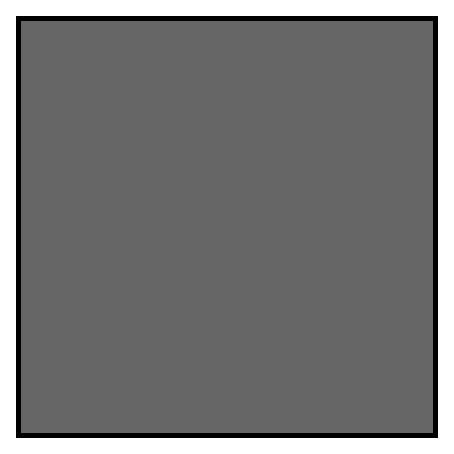
\includegraphics{example.eps}
%% figure caption is below the figure
%\caption{Please write your figure caption here}
%\label{fig:1}       % Give a unique label
%\end{figure}
%
% For two-column wide figures use
%\begin{figure*}
%% Use the relevant command to insert your figure file.
%% For example, with the graphicx package use
%  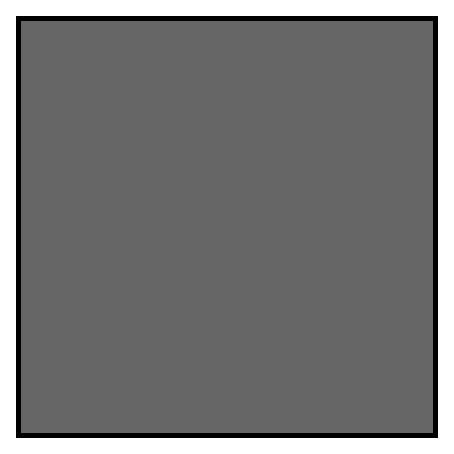
\includegraphics[width=0.75\textwidth]{example.eps}
%% figure caption is below the figure
%\caption{Please write your figure caption here}
%\label{fig:2}       % Give a unique label
%\end{figure*}
%
%% For tables use
%\begin{table}
%% table caption is above the table
%\caption{Please write your table caption here}
%\label{tab:1}       % Give a unique label
%% For LaTeX tables use
%\begin{tabular}{lll}
%\hline\noalign{\smallskip}
%first & second & third  \\
%\noalign{\smallskip}\hline\noalign{\smallskip}
%number & number & number \\
%number & number & number \\
%\noalign{\smallskip}\hline
%\end{tabular}
%\end{table}


%\begin{acknowledgements}
%If you'd like to thank anyone, place your comments here
%and remove the percent signs.
%\end{acknowledgements}

% BibTeX users please use one of
%\bibliographystyle{spbasic}      % basic style, author-year citations
\bibliographystyle{spmpsci}      % mathematics and physical sciences
%\bibliographystyle{spphys}       % APS-like style for physics
\bibliography{BibSources}   % name your BibTeX data base



%% Non-BibTeX users please use
%\begin{thebibliography}{}
%%
%% and use \bibitem to create references. Consult the Instructions
%% for authors for reference list style.
%%
%\bibitem{RefJ}
%% Format for Journal Reference
%Author, Article title, Journal, Volume, page numbers (year)
%% Format for books
%\bibitem{RefB}
%Author, Book title, page numbers. Publisher, place (year)
%% etc
%\end{thebibliography}

\end{document}
% end of file template.tex

